\documentclass[a4paper,11pt,parskip=half,cleardoublepage=empty]{scrbook}

\usepackage[english, ngerman]{babel}
\usepackage{lmodern}
\usepackage{xcolor}
\usepackage{tikz}
\usepackage{minted}
\usepackage{wrapfig}
\usepackage{graphicx}
\usepackage{eso-pic}
\usepackage[backend=biber,style=numeric]{biblatex}
\usepackage{hyperref}
\usepackage{booktabs}
\usepackage{amsmath}

\definecolor{uibkorange}{RGB}{246, 135, 18}
\definecolor{uibkgraym}{RGB}{123, 121, 121}
\definecolor{uibkblue}{RGB}{10, 38, 74}

\addbibresource{references.bib}

\graphicspath{{img/}}
\newcommand*{\xchapter}{\stepcounter{chapter}\setcounter{section}{0}\addchap}
\renewcommand*{\thesection}{\arabic{section}}

% define medatata
\def\MTitle{Increasing throughput of server applications by using asynchronous techniques: A case study on CoAP.NET}
\def\MAuthor{Philip Wille}
\def\MKeywords{TAP \sep C\#\sep CoAP\sep Server application}
\def\MOrg{Universität Innsbruck}
\def\MDate{\today}
\def\MInstitution{Department of Computer Science}
\def\MSupervisor{Dr. Michael Felderer}
\def\MGroup{Research Group Quality Engineering}

\begin{document}

    \frontmatter
\pagestyle{empty}

\begin{titlepage}
	\rule{0mm}{1mm}
	\vspace*{10mm}
%\begin{wrapfigure}{l}{3.25cm}
%    \includegraphics[width=3cm]{uni-logo-4c}
%\end{wrapfigure}
%\begin{flushright}
%    \setlength{\unitlength}{1cm}
%    {\large \MOrg \vskip 5mm
%    \MInstitution}\\
%    \textbf{\large \MGroup}
%    \vskip 15mm
%    \textbf{\Large S\,E\,M\,I\,N\,A\,R\,\,\,P\,A\,P\,E\,R}
%\end{flushright}

	\begin{center}
		\begin{figure}
			\centering
			
\includegraphics[width=7cm]{uni-innsbruck}
		\end{figure}	
		\vskip 25mm
		{\LARGE\textbf{\MTitle}}
		\vskip 5mm
		\vskip 1cm
		{\Large \textbf{\MAuthor}}\vskip 15mm
		\vskip 15mm
		\textbf{\large Bachelor Thesis}    
		\vskip 3cm
		{\large Supervisor:\\}
		{\MSupervisor\\}
		{\large \MInstitution\\}
		{\large \MOrg}    
		\vfill
		{\large Innsbruck, \MDate} 
	\end{center}
	\AddToShipoutPicture{
	\put(-55,55){
		\parbox[b]{\paperwidth}{
			\hfill 
\includegraphics[scale=0.35]{uni-watermark}
		}
	}
	}
\end{titlepage}

\ClearShipoutPicture

    \cleardoublepage
    \tableofcontents 
    \cleardoublepage
    \pagenumbering{arabic}
    \pagestyle{plain} 

    \section{Einleitung}
\label{sec:einleitung}

Heutzutage haben Webdienste einen hohen Stellenwert im Internet. Sie sind häufig ein essenzieller Bestandteil von Anwendungen und werden durch eine \textit{Representation State Transfer} (REST)-Schnittstelle für Anwender und Entwickler angeboten. Auch das \textit{Internet of Things} (IoT) bekommt mit fortschreitender Zeit eine immer wichtigere Rolle in der Entwicklung von Anwendungen, wie zum Beispiel in der Hausautomatisierung oder smarte Energieverwaltung, wie in den wissenschaftlichen Berichten \citetitle{HomeAutomationUsingCoAP} von \citeauthor{HomeAutomationUsingCoAP} \autocite{HomeAutomationUsingCoAP}, \citetitle{okur2014study} von \citeauthor{okur2014study} \autocite{okur2014study}, \citetitle{TinyCoAP} von \citeauthor{TinyCoAP} \autocite{TinyCoAP} oder \citetitle{TransportLogisticUsingCoAP} von \citeauthor{TransportLogisticUsingCoAP} \autocite{TransportLogisticUsingCoAP} thematisiert wird.

Um die REST-Architektur auch für eingeschränkte Geräte anbieten zu können, wurde mit \textit{Constrained RESTful Environments} (CoRE) eine geeignete Form geschaffen. Somit können solche Geräte, wie zum Beispiel 8-Bit-Mikrocontroller mit begrenztem Arbeitsspeicher und Readonly-Memory (ROM), als auch Netzwerke, wie zum Beispiel \textit{IPv6 over Low-Power Wireless Area Networks (6LoWPANs)}, solche Architekturen verwenden und realisieren. Damit eine Fragmentierung von Nachrichten in solchen Netzwerken so gering wie möglich auftritt, wird im Constrained Application Protocol (CoAP) ein so niedriger Nachrichten-Overhead wie möglich angestrebt.

Mit CoAP wurde die Entwicklung eines generischen Webprotokolls für die speziellen Anforderungen dieser eingeschränkten Umgebungen, insbesondere mit Hauptaugenmerk auf Energie-, Gebäudeautomatisierungs- und andere Machine-to-Machine (M2M) Anwendungen vorangetrieben. Dabei sollte CoAP keine komprimierte Abwandlung von \textit{Hypertext Transfer Protocol}, abgekürzt HTTP, sein, sondern vielmehr eine Submenge von HTTP mit Verwendung von REST, die für M2M-Szenarien optimiert ist. Somit könnte CoAP leicht dazu verwendet werden, einfache HTTP-Schnittstellen in ein kompaktes Protokoll überzuführen, jedoch bietet CoAP Funktionen an, die speziell in Machine-to-Machine-Anwendungen Verwendung finden. Diese Funktionen sind:
\begin{itemize}
    \item Eingebaute Entdeckung von, im Netzwerk, angebotenen Services und Ressourcen.
    \item Mutlicast-Unterstützung.
    \item Asynchroner Nachrichtenaustausch.
\end{itemize}

In den, von CoAP angedachten Anwendungsgebieten, in denen eine große Menge an Daten über ein Netzwerk fließen, könnten asynchrone Techniken die passende Ergänzung sein, um eine hohe Anzahl von Nachrichten zu empfangen, zu versenden oder zu verarbeiten. Den mit steigender Digitalisierung in privaten als auch geschäftlichem Umfeld, im Form von intelligenter Haussteuerung, effizienter Nutzung von Energieerzeugern und Energieverbrauchern\footnote{\href{https://www.a1energysolutions.at/smartspeicher/}{SmartSpeicher} - intelligente Warmwasserspeicher zur Stabilisierung des Stromnetzes}, steigt auch der Bedarf an leistungsfähigen Anwendungen, die diese schnell anwachsende Anzahl an IoT-Geräten ressourcenschonend und effizient verwalten kann. 

Jedoch eignet sich Asynchronität nicht nur zur Optimierung von Anwendungen im IoT-Bereich, sondern auch für solche mit einer grafischen Programmoberfläche (GUI). Dies hat den Grund, da der für das Zeichnen der Oberfläche verantwortliche Thread freibleibt und somit neu ankommende Eingaben des Benutzers (Mausklick, Tastatureingabe etc.) verarbeiten werden kann, ohne das die Oberfläche "einfriert"\footnote{Beschreibung des Zustandes eines Programmes, indem die Oberfläche keine neuen Eingaben entgegennimmt}.

Dieses Programmierparadigma ist auch nützlich, wenn mit Datenbanken oder REST-Schnittstellen interagiert oder I/O- bzw. CPU-intensive Operationen ausgeführt werden, wie \citeauthor{okur2014study} in deren Studie \citetitle{okur2014study} \autocite{okur2014study} herausgefunden haben.

\subsection{Constrained Application Protocol (CoAP)}
\label{subsec:constrained-application-protocol}

Das \textit{Constrained Application Protocol}, abgekürzt CoAP, ist ein Internetprotokoll, das speziell für M2M Anwendungen, wie zum Beispiel smarte Energieverwaltung oder Hausautomatisierung, entwickelt wurde \autocite{coap}. Dabei bietet das Protokoll ein REST-ähnliches Interface für Mikrocontroller mit angeschlossenen Aktoren oder Sensoren, auch \textit{constrained nodes} genannt, oder auch drahtlose Sensornetze, auch \textit{constrained networks} genannt, an. Die sogenannten \textit{nodes} besitzen meist einen angeschlossenen 8-Bit-Mikrocontroller, der nur eine kleine begrenzte Menge an Arbeitsspeicher (RAM) und Readonly-Memory (ROM) beinhaltet. Bei \textit{contstrained networks}, wie z.B. \textit{IPv6 over Low-Power Wireless Area Networks (6LoWPANs)}, spielt die hohe Paketverlustrate und der für solche Netzwerke typische Datendurchsatz von wenigen 10 kbit/s eine große Rolle. CoAP ist durch den RFC 7252 von \citeauthor{RFC7252} \cite{RFC7252} spezifiziert.

Dabei bietet das \textit{Constrained Application Protocol} ein Interaktionsmodell für Anfragen und Antworten zwischen den, in der Anwendung, definierten Endpunkten an. Auch ist eine eingebaute Entdeckung von, im Netzwerk, angebotenen Services und Ressourcen im Protokoll definiert. Zusätzlich werden Hauptbestandteile des Internets, wie \textit{Unique Resource Identifiers} (URIs) und \textit{Internet Media Types} (zum Beispiel \textit{application/json}) angeboten.

Eine Unterstützung von \textit{Multicast} ist gegeben, als auch ein sehr geringer Mehraufwand in der Datenübertragung. Ferner wurde darauf Wert gelegt, es einfach für eingebettete Systeme zu halten.

Zur Datenübertragung nutzt CoAP das \textit{User Datagram Protocol} (UDP). Dieses unterscheidet sich zum \textit{Transmission Control Protocol} (TCP) in den folgenden Punkten:
\begin{itemize}
    \item Kein Sitzungsaufbau von Sender zu Empfänger (\textit{Handshake}).
    \item Stellt nicht sicher, ob alle Pakete beim Empfänger eintreffen.
    \item Geht ein Paket verloren, wird dieses nicht erneut versendet.
\end{itemize}

Die folgenden Funktionen sind essenzielle Bestandteile von CoAP:
\begin{itemize}
    \item Erfüllung von M2M Anforderungen in eingeschränkten Umgebungen.
    \item UDP-Verbindung mit optionaler Zuverlässigkeit, die Unicast- und Multicast Anfragen unterstützt.
    \item Asynchroner Nachrichtenaustausch.
    \item Niedriger Mehraufwand durch veränderten Header und niedriger Komplexität des Parsings.
    \item URI- und Content-Typen-Support.
    \item Einfache Proxy- und Caching-Unterstützung.
    \item Zustandsloses HTTP-Mapping, welches die Entwicklung von Proxys erlaubt, die den Zugriff auf CoAP Ressourcen über HTTP auf einheitliche Weise ermöglichen oder für einfache HTTP-Schnittstellen, die alternativ über CoAP realisiert werden können.
    \item Sicherheitsmechanismen durch das Anbinden von \textit{Datagram Transport Layer Security} (DTLS).
\end{itemize}

\subsubsection{Begriffe in CoAP}
\label{subsubsec:begiffe-in-coap}

Um den Kontext innerhalb des \textit{Constrained Application Protocols} zu verstehen, werden nachfolgend die wichtigsten Begriffe in CoAP kurz erklärt:
\begin{itemize}
    \item Endpunkt (Endpoint):
          \begin{itemize}
              \item Ein Endpunkt lebt auf einen "Knoten". Ein Knoten ist vergleichbar mit dem Begriff "Host", der vorwiegend in anderen Internetstandards Erwähnung findet.
              \item Ein Endpunkt wird durch Multiplexing-Informationen auf der Transportschicht identifiziert, die eine UDP-Portnummer und eine Sicherheitszuordnung enthalten könnte.
          \end{itemize}
    \item Ursprungsserver (Origin Server):
          \begin{itemize}
              \item Jener Server, auf dem sich eine bestimmte Ressource befindet oder erstellt werden soll.
          \end{itemize}
    \item Bestätigende Nachricht (Confirmable Message):
          \begin{itemize}
              \item Einige Nachrichten benötigen eine Bestätigung des Empfängers. Diese Nachrichten werden als \textit{bestätigt} behandelt.
              \item Falls keine Pakete während der Übertragung verloren gingen, wird für jede Nachricht, die bestätigt werden muss, exakt eine Nachricht des Typs \textit{Acknowledgement} oder \textit{Reset} an den Sender zurückgesendet.
          \end{itemize}
    \item Nicht bestätigende Nachricht (Non-confirmable Message):
          \begin{itemize}
              \item Im Gegensatz zu bestätigenden Nachrichten gibt es auch Nachrichten, die nicht bestätigt werden müssen.
              \item Dies betrifft Nachrichten, die für bestimmte Anwendungsanforderungen häufiger wiederholt werden müssen, wie zum Beispiel, das wiederholte Lesen eines Sensors.
          \end{itemize}
    \item Bestätigungsnachricht (Acknowledgement Message):
          \begin{itemize}
              \item Eine solche Nachricht bestätigt den Empfang einer bestätigenden Nachricht. Eine Bestätigungsnachricht sagt nicht aus, ob die Anfrage, die mit einer bestätigenden Nachricht versendet wurde, erfolgreich war oder nicht.
              \item Jedoch enthält die Bestätigungsnachricht auch eine sogenannte \textit{Piggybacked Response}.
          \end{itemize}
    \item Rücksetzende Nachricht (Reset message):
          \begin{itemize}
              \item Diese Nachricht sagt aus, dass eine spezifische Nachricht, mit dem Typ \textit{Confirmable} oder \textit{Non-confirmable}, empfangen wurde, jedoch einige Teile des Nachrichtenkontextes fehlen, um diese Nachricht korrekt verarbeiten zu können.
              \item Dieses Verhalten tritt auf, wenn der zu empfangende Endpunkt neu gestartet wurde und somit den Zustand vergessen hat, der zur vollständigen Interpretation der Nachricht nötig war.
              \item Ein absichtliches Provozieren einer rücksetzenden Nachricht \textit{Reset Message}, zum Beispiel durch das Senden einer leeren bestätigenden Nachricht (\textit{Empty Confirmable Message}), kann als eine kostengünstige Prüfung der Funktionsfähigkeit eines Endpunktes verwendet werden - vergleichbar mit einem \textit{Ping}.
          \end{itemize}
    \item \textit{"Antwort im Huckepackverfahren"} (Piggybacked Response):
          \begin{itemize}
              \item Eine \textit{Piggybacked Response} ist direkt in eine \textit{Acknowledgement} (ACK) Nachricht inkludiert, die gesendet wird, um den Empfang der Anfrage für diese Antwort zu bestätigen.
          \end{itemize}
    \item Separate Antwort (Separate Response):
          \begin{itemize}
              \item Wenn eine \textit{Confirmable} Nachricht mit einer Anfrage mit einer \textit{Empty} Nachricht quittiert wird (z.B. weil der Server die Antwort nicht sofort hat), wird eine separate Antwort in einem separaten Nachrichtenaustausch gesendet.
          \end{itemize}
    \item Leere Nachricht (Empty Message):
          \begin{itemize}
              \item Eine Nachricht mit dem Code 0.00. Die Nachricht ist weder eine Anfrage noch eine Antwort. Sie beinhaltet nur den 4-Byte-langen Kopf (\textit{header}).
          \end{itemize}
\end{itemize}

\subsubsection{Nachrichtenübertragung}
\label{subsubsec:nachrichtenuebertragung}

CoAP nutzt zur Nachrichtenübertragung UDP, um den Austausch von Nachrichten asynchron ausführen zu können. Dies wird dadurch erreicht, dass eine weitere Schicht auf UDP aufbauend eingefügt wird (siehe Ababbildungung \ref{fig:abstrakte-darstellung-der-verschiedenen-schichten}). Diese Schicht kann optional auch einen Mechanismus zur Sicherstellung des Nachrichtenaustausches beinhalten. Dabei definiert CoAP vier verschiedene Arten von Nachrichten:
\begin{itemize}
    \item Bestätigende Nachricht (\textit{Confirmable Message}),
    \item Nicht bestätigende Nachricht (\textit{Non-confirmable Message}),
    \item Bestätigungsnachricht (\textit{Acknowledgement Message}),
    \item Rücksetzende Nachricht (\textit{Reset Message}),
\end{itemize}

Diese vier Arten stehen orthogonal zueinander, sprich:
\begin{itemize}
    \item Bestätigende und nicht bestätigende Nachrichten sind für Anfragen (\textit{requests}) gedacht.
    \item Rücksetzende Nachrichten oder Nachrichten, die eine Anfrage bestätigen, sind für Antworten (\textit{responses}) gedacht.
\end{itemize}

\begin{figure}[h]
    \centering
    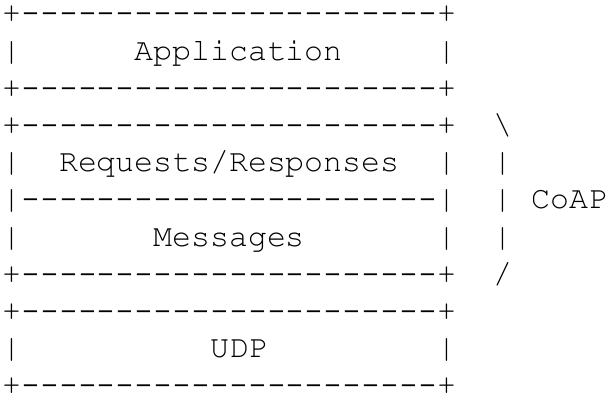
\includegraphics[width=0.5\textwidth]{abstract_layering_of_coap}
    \caption{Abstrakte Darstellung der verschiedenen Schichten (Quelle: RFC 7252 \autocite{RFC7252})}
    \label{fig:abstrakte-darstellung-der-verschiedenen-schichten}
\end{figure}

Das Nachrichtenmodell des Constrained Application Protocols basiert auf den Austausch von Nachrichten über UDP. Dabei beginnt die Nachricht mit einer in der Länge fixierten Vier-Byte-Langen Kopfzeile (\textit{header}), gefolgt von einem optionalen Token (null bis acht Bytes lang), und null oder mehr sogenannten Optionen. Diese Optionen sind vergleichbar mit den \textit{header fields} von HTTP. Nach den Optionen befindet sich ein sogenannter Anhang-Markierer (\textit{Payload marker}), der einem Byte mit acht logischen Einsen, hexadezimal auch 0xFF kodiert, entspricht, jedoch nur in der Nachricht enthalten ist, wenn eine Payload mitgesendet wird. Anschließend an den \textit{Payload marker} kommt der Anhang (\textit{Payload}). Dieses Format ist sowohl für Anfragen als auch für Antworten dasselbe.

Damit Nachrichten als eindeutig identifiziert werden können, wird ein sogenannter Nachrichtenbezeichner (\textit{Message ID}) verwendet. Dieser ist 16 Bit lang und erlaubt somit, bei Implementierungen mit Standardeinstellungen, bis zu 250 Nachrichten die Sekunde von einem Endpunkt zu einem anderen zu senden. Die \textit{Message ID} wird auch für die Sicherstellung des Nachrichtenaustausches (\textit{reliability}) benötigt. Dabei ist jedoch die \textit{Message ID} nur zwischen zwei Endpunkten eindeutig. Kommuniziert ein Teilnehmer mit mehreren Teilnehmern gleichzeitig, dann können die \textit{Message IDs} häufiger vorkommen. Für die eindeutige Identifizierung der Kommunikation zwischen zwei Teilnehmern wird der sogenannte Token verwendet. Dieser ist über mehrere Verbindungen hinweg eindeutig und kann als Identifikator für derzeit laufende Verbindungen gesehen werden.

Die Sicherstellung des Nachrichtenaustausches erfolgt dadurch, dass man eine Nachricht als bestätigend (\textit{Confirmable}) markiert. Eine als \textit{Confirmable} gekennzeichnete Nachricht wird so lange an den jeweiligen Empfänger gesendet, bis dieser eine \textit{Acknowledgement} Nachricht mit derselben \textit{Message ID} zurücksendet (wie in Abbildung \ref{fig:nachrichtenaustausch-mit-sicherstellung-des-transfers} dargestellt). Wenn der Empfänger die \textit{Confirmable} Nachricht, aufgrund fehlender Daten oder fehlendem Kontext nicht beantworten kann, sendet dieser eine \textit{Reset} Nachricht zurück.

\begin{figure}[h]
    \centering
    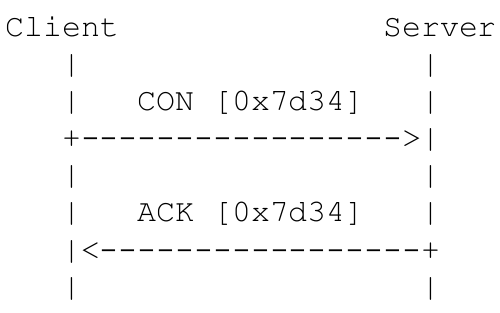
\includegraphics[width=0.5\textwidth]{reliable_message_transmission}
    \caption{Nachrichtenaustausch mit Sicherstellung des Transfers (Quelle: RFC 7252 \autocite{RFC7252})}
    \label{fig:nachrichtenaustausch-mit-sicherstellung-des-transfers}
\end{figure}

Jedoch wird für den Austausch von Nachrichten im CoAP Kontext kein Sicherheitsmechanismus für die Übertragung gefordert, sondern es können auch Nachrichten als \textit{Non-confirmable} markiert werden (siehe Abbildung \ref{fig:nachrichtenaustausch-ohne-sicherstellung-des-transfers}). Diese Vorgangsweise bietet sich zum Beispiel an, wenn man die Messdaten eines Sensors wiederholt ausliest. Dabei werden \textit{Non-confirmable} Nachrichten nicht bestätigt, jedoch wird eine \textit{Message ID} benutzt, um Duplikate zu erkennen.

\begin{figure}[h]
    \centering
    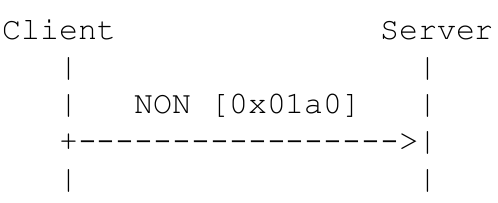
\includegraphics[width=0.5\textwidth]{unreliable_message_transmission}
    \caption{Nachrichtenaustausch ohne Sicherstellung des Transfers (Quelle: RFC 7252 \autocite{RFC7252}).}
    \label{fig:nachrichtenaustausch-ohne-sicherstellung-des-transfers}
\end{figure}

Kann eine ankommende Anfrage (\textit{Request}), welche mithilfe einer \textit{Confirmable} Nachricht versendet wurde, sofort beantwortet werden, wird die Antwort (\textit{Response}) in der daraus resultierenden \textit{Acknowledgment} Nachricht zurückgesendet. Dieses Prinzip nennt man auch \textit{Piggybacked Response}. Das Abbildung \ref{fig:beispiel-eines-erfolgreichen-piggybacked-response} stellt diesen Mechanismus dar.

\begin{figure}[h]
    \centering
    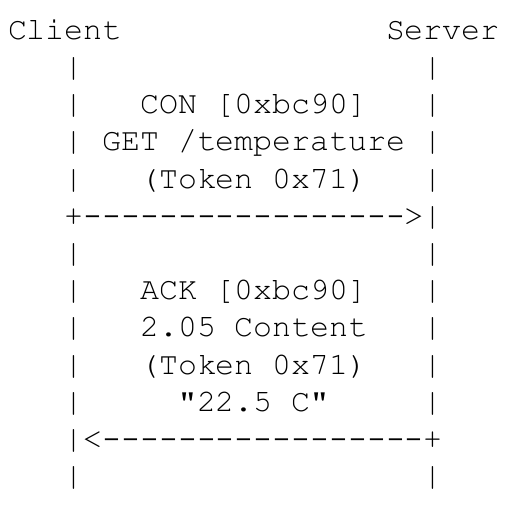
\includegraphics[width=0.5\textwidth]{piggybacked_response}
    \caption{Beispiel einer erfolgreichen \textit{Piggybacked Response} (Quelle: RFC 7252 \cite{RFC7252}).}
    \label{fig:beispiel-eines-erfolgreichen-piggybacked-response}
\end{figure}

Ist der Server jedoch nicht sofort in der Lage die Anfrage zu beantworten, dann antwortet dieser mit einer leeren \textit{Confirmable} Nachricht. Dies macht er, um den Client am wiederholten Senden der Anfrage zu hindern. Sind alle benötigten Daten zur Beantwortung der Anfrage vorhanden, sendet der Server die Antwort in einer neuen \textit{Confirmable} Nachricht zurück. Dieses Prinzip wird als separate Antwort (\textit{separate response}) bezeichnet und wird in der Abbildung \ref{fig:beispiel-einer-separate-response} dargestellt.

\begin{figure}[h]
    \centering
    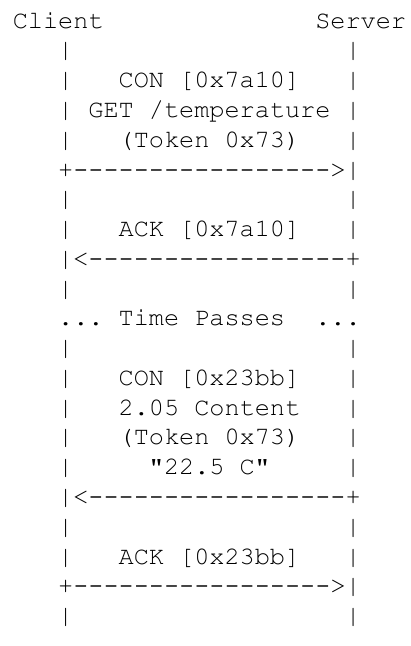
\includegraphics[width=0.5\textwidth]{separate_response}
    \caption{Beispiel einer \textit{separate response} (Quelle: RFC 7252 \cite{RFC7252})}
    \label{fig:beispiel-einer-separate-response}
\end{figure}

Dabei macht CoAP von den bekannten Internetmethoden \textit{GET}, \textit{PUT}, \textit{POST} und \textit{DELETE} in einer ähnlichen Art gebrauch, wie es HTTP macht.

\subsubsection{Nachrichtenformat}
\label{subsubsec:nachrichtenformat}

Wie schon erwähnt, basiert der Nachrichtenaustausch von CoAP auf UDP. Dabei nimmt jede, über UDP versendete Nachricht ein ganzes UDP Datagramm in Anspruch. Der Aufbau einer CoAP Nachricht ist einfach gehalten und startet mit einer Vier-Byte-langen-Kopfzeile (\textit{Header}), welche folgenden Daten beinhaltet, visualisiert in Abbildung \ref{fig:binaere-sturktur-eines-coap-headers}:
\begin{itemize}
    \item \textit{Version}
    \item \textit{Type}
    \item \textit{Token Length}
    \item \textit{Code}
    \item \textit{Message ID}
\end{itemize}

Dabei repräsentieren die ersten zwei Bits des \textit{Headers} die Versionsnummer. Die Versionsnummer gibt an, in welcher CoAP Version die Nachricht erstellt wurde bzw. verarbeitet werden kann. In dieser Arbeit beschäftigen wir uns mit CoAP Nachrichten mit der Versionsnummer 1, in Binär als 01 kodiert.

Die darauffolgenden zwei Bits entsprechen dem Typ der CoAP Nachricht. Der Typ gibt an, ob es sich um eine \textit{Confirmable} (0 = in Binär als 00 kodiert), \textit{Non-Confirmable} (1 = 01), \textit{Acknowledgement}  (2 = 10) oder \textit{Reset} (3 = 11) Nachricht handelt.

Als Nächstes kommt die vier Bit lange \textit{Token Length}, welche die Länge des \textit{Tokens} angibt. Dabei kann der \textit{Token} zwischen null, in Binär als 0000 kodiert, und acht, in Binär als 0111 kodiert, Bytes lang sein. \textit{Token Lengths}, welche zwischen neun und fünfzehn Bytes lang sind, sind im RFC 7252 \autocite{RFC7252} für zukünftige Versionen reserviert.

Die nächsten acht Bit geben den \textit{Code}, vergleichbar mit dem Statuscode bei HTTP, der CoAP Nachricht an. Dabei unterteilt sich der \textit{Code} in eine drei Bit lange \textit{Code Class} (\textit{most significant bits}) und einen fünf Bit langen \textit{Code Detail} (\textit{least significatn bits}). Dabei folgt der \textit{Code} dem Schema "c.dd", wobei "c" Werte von 0 bis 7 annehmen kann und "dd" Werte von 00 bis 31. Die \textit{Code Class} gibt dabei an, ob es sich um
\begin{itemize}
    \item eine Anfrage (0),
    \item eine erfolgreiche Antwort (2),
    \item eine clientseitige, fehlerhafte Antwort (4),
    \item oder eine serverseitige, fehlerhafte Antwort (5) handelt.
\end{itemize}

Daneben nimmt der \textit{Code} 0.00 eine besondere Stellung ein, da dieser eine leere Nachricht (\textit{Empty Message}) markiert. Die \textit{Codes} gleichen sich mit einigen Statuscodes, welche man von HTTP kennt, jedoch ist nicht jeder Statuscode als CoAP \textit{Code} abgebildet.

Der letzte Teil des \textit{Headers} ist die sogenannte \textit{Message Id}, die 16 Bit in Anspruch nimmt und in der \textit{Network Byte Order}, auch unter dem Begriff \textit{Big Endian} bekannt, angegeben wird. Dessen Aufgabe ist es, Duplikate von Nachrichten zu erkennen. Auch wird die \textit{Message Id} dafür benutzt, um Nachrichten vom Typ \textit{Acknowledgement} und \textit{Reset} zu Nachrichten vom Typ \textit{Confirmable} und \textit{Non-Confirmable} zu verlinken. Somit besitzt der Server immer einen Überblick, zu welcher Anfrage schon eine Antwort geschickt wurde.

\begin{figure}[h]
    \centering
    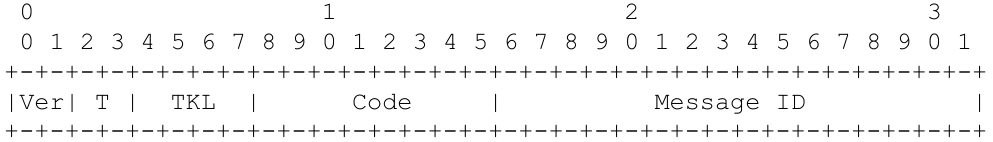
\includegraphics[width=0.75\textwidth]{coap_header}
    \caption{Binäre Struktur eines CoAP \textit{Headers} (Quelle: RFC 7252 \autocite{RFC7252})}
    \label{fig:binaere-sturktur-eines-coap-headers}
\end{figure}

Anschließend an den \textit{Header} kommt der \textit{Token} der Nachricht. Dieser ist in seiner Länge variabel und hängt von der im \textit{Header} angegebenen \textit{Token Length} ab. Dieser ist zuständig für die Korrelation von Anfragen zu Antworten.

Nachfolgend können null oder mehr sogenannte \textit{Options} folgen. Der Option können folgende Bestandteile einer CoAP Nachricht folgen:
\begin{itemize}
    \item Das Ende der CoAP Nachricht (EoF),
    \item Eine weitere Option,
    \item Oder der \textit{Payload Marker} mit anschließender \textit{Payload}.
\end{itemize}

Ist eine \textit{Payload} gegeben, folgt nach der Gruppe von Optionen ein sogenannter \textit{Payload Marker}. Dieser besteht aus einem Byte voller logischer Einsen, hexadezimal als 0xFF kodiert, und markiert somit das Ende der \textit{Options}. Alle Daten, die sich nach dem \textit{Payload Marker} befinden, werden als \textit{Payload} interpretiert. Dabei ist die Länge durch die \textit{UDP Datagram} Paketgröße von 65 535 Bytes begrenzt. Werden für die Übertragung der Nachricht mehr Bytes benötigt als ein \textit{UDP Datagram} an Größe bereitstellen kann, werden die Bytes auf mehrere \textit{UDP Datagrams} aufgeteilt. Diesen Mechanismus nennt man auch \textit{Blockwise transfer} und wird im RFC 7959 von \citeauthor{RFC7959} \cite{RFC7959}, der auf dem RFC 7252 von \citeauthor{RFC7252} \autocite{RFC7252} aufbaut, beschrieben.

\begin{figure}[h]
    \centering
    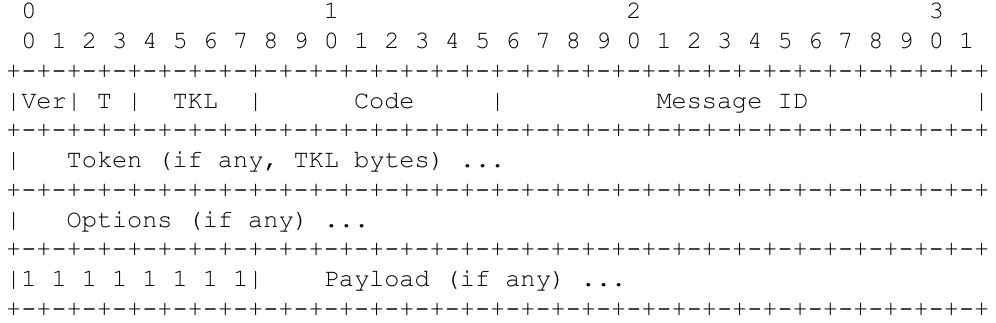
\includegraphics[width=0.75\textwidth]{coap_message}
    \caption{Binäre Struktur einer vollständigen CoAP Nachricht (Quelle: RFC 7252 \autocite{RFC7252})}
    \label{fig:binaere-sturktur-einer-vollstaendigen-coap-nachricht}
\end{figure}

\subsubsection{Aufbau einer Option}
\label{subsubsec:aufbau-einer-option}

Eine Option wird durch eine eindeutige Nummer identifiziert. Neben der Nummer besitzt eine Option auch einen Wert (\textit{Value}), den diese Option hält, und einen Indikator für die Länge des Wertes. Dabei wird die Nummer nicht direkt in die Nachricht kodiert, sondern die Optionen werden zuerst aufsteigend nach ihrer Nummer sortiert und dann wird eine Deltakodierung (Differenzbildung) zwischen der aktuellen Option und deren Vorgängern gebildet. Dies geschieht dadurch, dass alle vorherigen Differenzen, auch im RFC 7252 \autocite{RFC7252} als \textit{Delta} bezeichnet, addiert werden und dann die Differenz zur aktuellen Option gebildet wird. Für die erste Option wird der Sonderfall behandelt, dass als vorheriges Delta ein Wert von null angenommen wird. Dies resultiert daraus, dass für die erste Option die kodierte Differenz als Nummer der Option verwendet wird. Ein weiterer Sonderfall ist derjenige, wenn mehrere Instanzen der gleichen Option in der Kollektion von Optionen auftritt. Dabei ist die Differenz zwischen zwei gleichen Optionen immer null.

Eine Option fängt immer mit einem Byte an, das zwei Informationen enthält. Einmal die Differenz (\textit{Option Delta}) und andererseits die Länge des Wertes (\textit{Option Length}) der Option. Das \textit{Option Delta} entspricht dabei den ersten vier Bits (\textit{most significant bits}) und die \textit{Option Length} den letzten vier Bits (\textit{least significant bits}). Man kann dieses Byte auch als einen \textit{Header} für Options bezeichnen, da dieser Informationen beinhaltet, die für das Kodierung bzw. Dekodieren von Options benötigt wird.

Um jedoch Deltas und Längen, jenseits des Wertes fünfzehn, verwenden zu können, können dem \textit{Option Header} das \textit{Option Delta (extended)} und die \textit{Option Length (extended)} folgen. Diese beiden können jeweils zwischen null und zwei Bytes lang sein. Nach diesen beiden folgt der sogenannte \textit{Option Value}, der null oder mehr Bytes betragen kann.

\begin{figure}[h]
    \centering
    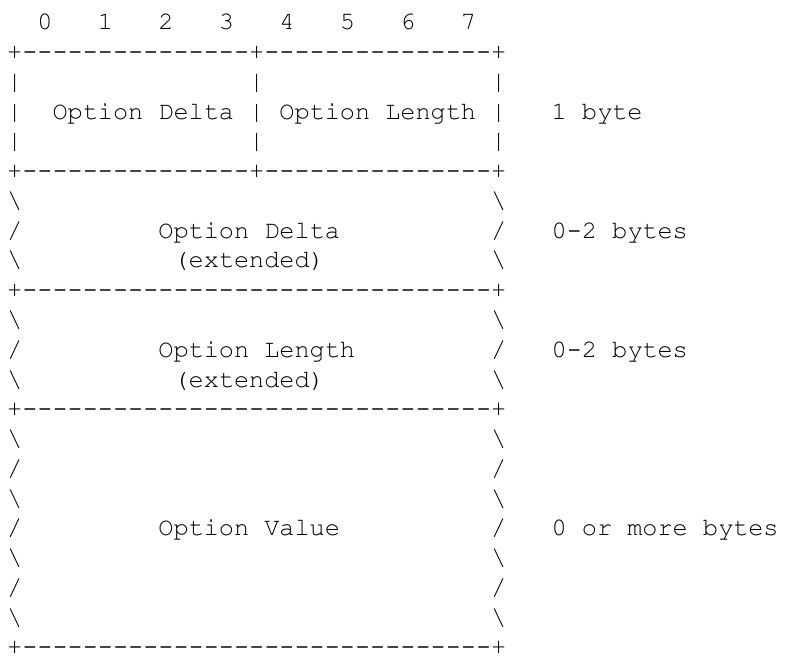
\includegraphics[width=0.75\textwidth]{structure_option.png}
    \caption{Binäre Struktur einer CoAP-Option (Quelle: RFC 7252 \autocite{RFC7252})}
    \label{fig:binaere-sturktur-einer-coap-option}
\end{figure}

\subsection{Ausführungsparadigmen in der Informatik}
\label{subsubsec:ausfuehrungsparadigmen-in-der-informatik}

In der Informatik spricht man von zwei großen Ausführungsparadigmen, mit denen Programme bzw. Codeteile ausgeführt werden können: \textbf{synchrone} und \textbf{asynchrone Ausführung}. Diese beiden Ausführungsparadigmen unterscheiden sich in wesentlichen Punkten deutlich voneinander und bieten in verschiedenen Einsatzszenarien Vor- und Nachteile (siehe Tabelle \ref{tab:vergleich-synchroner-asynchroner-Ausfuehrung}). Dabei unterstützen die geläufigsten Programmiersprachen von Haus aus eine synchrone Ausführung von Programmen, jedoch bieten nicht alle eine asynchrone Ausführung.

\begin{table}[h]
    \resizebox{\textwidth}{!}{%
        \begin{tabular}{@{}lll@{}}
            \toprule
                          & Synchron                                       & Asynchron                                       \\ \midrule
            Programmfluss & Stoppt den Programmfluss.                      & Kann im Programmfluss weiter gehen.             \\ \midrule
            Beendigung    & Überprüft periodisch, ob Funktion beendet ist. & Ein Event markiert die Beendigung der Funktion. \\ \midrule
            Main-Thread   & Ist als "Blocked" oder "Waiting" markiert.     & Ist frei für andere Aufgaben.                   \\ \bottomrule
        \end{tabular}%
    }
    \caption{Vergleich zwischen synchroner und asynchroner Ausführung}
    \label{tab:vergleich-synchroner-asynchroner-Ausfuehrung}
\end{table}

Um diese Unterschiede zwischen den beiden Paradigmen zu veranschaulichen, wird dies anhand einer Client-Server-Anwendung mit einer an den Server angeschlossenen Datenbank und zwei Clients verbildlicht (siehe Abbildungen \ref{figure:sequendiagramm-eines-synchronen-servers} und \ref{figure:sequendiagramm-eines-asynchronen-servers}). Dabei ist der Server eine einfache Web-Applikation, welcher die Daten mittels SQL von der angeschlossenen Datenbank holt.

Senden nun beide Clients, in kurzem Zeitabstand zueinander, eine Anfrage an den Server, so kann der synchrone Server nur die Anfrage bearbeiten, die zuerst eintrifft - in diesem Fall die des Client 1. Dies geschieht deswegen, da der Main-Thread bzw. der für das Empfangen der Pakete zuständige Thread auf die Rückantwort des Datenbankservers wartet. Dadurch wird die Anfrage von Client 2 auf dem Server zurückgehalten und erst bearbeitet, wenn die erste Anfrage bearbeitet und zurückgesendet wurde. Dieses Verhalten skaliert schlecht mit mehreren, gleichzeitig eintreffenden Anfragen, da der sogenannte \textit{Threadpool}\footnote{Entspricht einer Queue in der die zu bearbeitenden Aufgaben abgelegt werden.}, bei zu vielen, langandauernden Anfragen, seine Kapazitätsgrenze erreicht und somit keine neuen Anfragen / Aufgaben annehmen kann.

\begin{figure}[ht]
    \centering
    \begin{tikzpicture}
        \node at (0,.3) {Database};
        \node at (-3,.3) {Server};
        \node at (-6,.3) {Client 2};
        \node at (-9,.3) {Client 1};

        \draw[thick, uibkorange] (-9,0) -- node[left] {prepare}(-9,-0.5);
        \draw[thick, uibkgraym] (-6,0) -- (-6,-0.5);
        \draw[thick, uibkgraym] (-3,0) -- (-3,-0.5);
        \draw[thick, uibkgraym] (-0,0) -- (0,-0.5);
        \draw[->, thick, uibkorange] (-9,-0.5) -- node[midway,above] {Request 1} (-3,-0.5);
        \draw[thick, uibkorange] (-3,-0.5) -- node[left] {prepare SQL}(-3,-1);
        \draw[->, thick, uibkorange] (-3,-1) -- node[midway,above] {SQL Request 1} (-0,-1);
        \draw[thick, uibkgraym] (0, -0.5) -- (0, -1);
        \draw[thick, uibkorange] (-0,-1) -- node [right] {execute} (0,-3);
        \draw[thick, uibkgraym] (-6, -0.5) -- (-6, -1);
        \draw[thick, uibkblue] (-6, -1) -- node[left] {prepare} (-6, -1.5);
        \draw[->, thick, uibkblue] (-6,-1.5) -- node[midway,above] {Request 2} (-3,-1.5);
        \draw[thick, uibkgraym] (-3,-1) -- (-3,-1.5);
        \draw[<-, thick, uibkorange] (-3,-3) -- node [midway, above] {SQL Response 1} (0,-3);
        \draw[thick, uibkgraym] (-3,-1.5) -- (-3,-3);
        \draw[thick, uibkorange] (-3,-3) -- (-3,-3.5);
        \draw[<-, thick, uibkorange] (-9,-3.5) -- node [midway, above] {Response 1} (-3,-3.5);
        \draw[thick, uibkgraym] (-9,-0.5) -- (-9,-3.5);
        \draw[thick, uibkorange] (-9,-3.5) -- node [midway, left] {process} (-9,-5.5);
        \draw[thick, uibkblue] (-3,-3.5) -- node [midway, left] {prepare SQL} (-3,-4);
        \draw[thick, uibkgraym] (-0,-3) -- (-0,-4);
        \draw[->, thick, uibkblue] (-3,-4) -- node [midway, above] {SQL Request 2} (-0,-4);
        \draw[thick, uibkblue] (-0,-4) -- node [midway, right] {execute} (-0,-5);
        \draw[thick, uibkgraym] (-3,-4) -- (-3,-5);
        \draw[<-, thick, uibkblue] (-3,-5) -- node [midway, above] {SQL Response 2} (-0,-5);
        \draw[thick, uibkblue] (-3,-5) -- (-3,-5.5);
        \draw[thick, uibkgraym] (-6,-1.5) -- (-6,-5.5);
        \draw[<-, thick, uibkblue] (-6,-5.5) -- node [midway, above] {Response 2} (-3,-5.5);
        \draw[thick, uibkgraym] (0, -5) -- (0, -5.5);
    \end{tikzpicture}
    \caption{Sequenzdiagramm eines synchronen Servers}
    \label{figure:sequendiagramm-eines-synchronen-servers}
\end{figure}

Setzt man anstelle eines synchronen Servers einen asynchronen Server ein, so ändert sich das beschriebene Szenario folgendermaßen: Trifft die Anfrage des Client 1 ein, wird diese, wie zuvor, sofort abgearbeitet. Dies geschieht jedoch auf einen anderen Thread, damit der Main-Thread bzw. der für das Empfangen der Pakete zuständige Thread wieder frei wird. Wird nun vom Client 2 eine Anfrage verschickt, dann kann der Server diese entgegennehmen und auf einen weiteren, freien Thread verlagern und bearbeiten. Je nachdem welche Anfrage schneller vom Datenbankserver verarbeitet wird, in diesem Fall die des Client 1, wird der Main-Thread bzw. der Thread, der das Paket zuvor entgegengenommen hat, über die Beendigung der Datenbankanfrage benachrichtigt. Somit kann dieser Thread seinen Kontext synchronisieren und die Antwort an den Client 1 zurücksenden.

Dieses Verfahren skaliert deutlich besser mit steigender Anzahl von Anfragen, jedoch kann dies auch mehr CPU- und Speicherressourcen verursachen. Dies liegt daran, dass zum Aufrechterhalten des Zustandes eine asynchrone Zustandsmaschine konstruiert wird und der Kontextwechsel bei Beendigung des asynchronen Aufrufs mit den Main-Thread synchronisiert werden muss.

\begin{figure}[ht]
    \centering
    \begin{tikzpicture}
        \node at (0,.3) {Database};
        \node at (-3,.3) {Server};
        \node at (-6,.3) {Client 2};
        \node at (-9,.3) {Client 1};
        
        \draw[thick, uibkorange] (-9,0) -- node[left] {prepare}(-9,-0.5);
        \draw[thick, uibkgraym] (-6,0) -- (-6,-0.5);
        \draw[thick, uibkgraym] (-3,0) -- (-3,-0.5);
        \draw[thick, uibkgraym] (-0,0) -- (0,-0.5);
        \draw[->, thick, uibkorange] (-9,-0.5) -- node[midway,above] {Request 1} (-3,-0.5);
        \draw[thick, uibkorange] (-3,-0.5) -- node[left] {prepare SQL}(-3,-1);
        \draw[thick, uibkgraym] (-6,-0.5) -- (-6,-1.5);
        \draw[->, thick, uibkorange] (-3,-1) -- node[midway,above] {SQL Request 1} (-0,-1);
        \draw[thick, uibkgraym] (0, -0.5) -- (0, -1);
        \draw[thick, uibkorange] (-0,-1) -- node [right] {execute} (0,-3);
        \draw[thick, uibkgraym] (-3,-1) -- (-3,-1.5);
        \draw[->, thick, uibkblue] (-6,-1.5) -- node[midway,above] {Request 2} (-3,-1.5);
        \draw[thick, uibkblue] (-3,-1.5) -- node[midway, left] {prepare SQL} (-3,-2);
        \draw[->, thick, uibkblue] (-3,-2) -- node [midway, above] {SQL Request 2} (-0,-2);
        \draw[thick, uibkgraym] (-3,-2) -- (-3,-3);
        \draw[<-, thick, uibkorange] (-3,-3) -- node [midway, above] {SQL Response 1} (0,-3);
        \draw[thick, uibkorange] (-3,-3) -- (-3,-3.5);
        \draw[<-, thick, uibkorange] (-9,-3.5) -- node [midway, above] {Response 1} (-3,-3.5);
        \draw[thick, uibkgraym] (-9,-0.5) -- (-9,-3.5);
        \draw[thick, uibkblue] (-0,-3) -- node [midway, right] {execute} (-0,-4);
        \draw[thick, uibkorange] (-9,-3.5) -- node [midway, left] {process} (-9,-5.5);
        \draw[thick, uibkgraym] (-3,-3.5) -- (-3,-4);
        \draw[<-, thick, uibkblue] (-3,-4) -- node [midway, above] {SQL Response 2} (-0,-4);
        \draw[thick, uibkblue] (-3,-4) -- (-3,-4.5);
        \draw[thick, uibkgraym] (0,-4) -- (0,-5.5);
        \draw[<-, thick, uibkblue] (-6,-4.5) -- node [midway, above] {Response 2} (-3,-4.5);
        \draw[thick, uibkgraym] (-6,-1.5) -- (-6,-4.5);
        \draw[thick, uibkblue] (-6,-4.5) -- node [midway, left] {process} (-6,-5.5);
        \draw[thick, uibkgraym] (-3,-4.5) -- (-3,-5.5);
    \end{tikzpicture}
    \caption{Sequenzdiagramm eines asynchronen Servers}
    \label{figure:sequendiagramm-eines-asynchronen-servers}
\end{figure}

\subsubsection{Asynchronität in C\#}
\label{subsubsec:ansynchronitaet-in-csharp}

Mit \textit{Task-based Asynchronous Pattern} (TAP) ermöglicht Microsoft in C\# Asynchronität. Dieses Pattern ermöglicht eine einfache Transformation von synchronen Code zu asynchronen Code ohne große Änderungen vornehmen zu müssen. Auch ist es von Haus aus im Sprachkonstrukt von C\# integriert und kann somit ohne zusätzliche Konfiguration verwendet werden.

Dabei baut das asynchrone Ausführungsparadigma für C\# auf folgende Komponenten auf:
\begin{itemize}
    \item \mintinline{csharp}{Task}: Ermöglicht eine asynchrone Methode zu definieren.
    \item \mintinline{csharp}{Task<TResult>}: Ermöglicht einen Rückgabewert vom Typ TResult von einer asynchronen Methode zurückzugeben.
    \item \mintinline{csharp}{CancellationToken}: Ermöglicht es einen Aufruf einer asynchronen Methode vorzeitig zu beenden.
    \item \mintinline{csharp}{async}/\mintinline{csharp}{await}: Schlüsselwörter um asynchrone Methoden zu deklarieren und auszuführen.
\end{itemize}

Im nachfolgenden Listing \ref{listing:synchrone-methode-in-csharp} wird eine Instanz eines DownloadClient erzeugt. Dieser besitzt eine Methode \textit{Download}, mit welcher der Inhalt einer Webseite heruntergeladen und als \mintinline{csharp}{string} zurückgegeben werden kann.

\begin{listing}[H]
    \inputminted[framesep=2mm, baselinestretch=1.2, fontsize=\normalsize, linenos]{csharp}{codes/example_synchronous.cs}
    \caption{Synchrone Methode in C\#}
    \label{listing:synchrone-methode-in-csharp}
\end{listing}

Diese Vorgehensweise hat den Nachteil, dass die Funktion den Main-Thread bzw. den Thread, der diese Methode aufgerufen hat, solange blockiert bis der gesamte Webseiteninhalt der angegebenen URI heruntergeladen wurde. Bei UI-Anwendungen lässt sich dadurch die Oberfläche nicht mehr bedienen und friert ein. Bei Verwendung in einer Konsolen-Applikation ohne UI ist der Main-Thread bis auf Weiteres blockiert und somit können andere Programmteile, die nicht auf das Ergebnis dieser Methode angewiesen sind, nicht ausgeführt werden.

Damit der aufzurufende Thread bzw. der Main-Thread nicht andauernd auf die Beendigung der Methode warten muss, kann man Events einsetzen, wie in Listing \ref{listing:eventbasierte-methode-in-csharp} dargestellt. Diese beendigen vorzeitig die Exekution der Methode, indem der Aufrufer ein Objekt übergeben bekommt. Dieses Objekt repräsentiert den derzeitigen Zustand der Operation - also in diesem Fall das Herunterladen des Webseiteninhaltes. Dafür wird in Zeile 3 das \mintinline{csharp}{DownloadResult}-Objekt erzeugt. In Zeile 5 wird durch den Operator \mintinline{csharp}{+=} die nachfolgende anonyme Lambdafunktion \mintinline{csharp}{(content) => result.SetComplete(content)} als Beobachter des Events \mintinline{csharp}{client.DownloadComplete} registriert. Diese Lambdafunktion hat die Aufgabe den heruntergeladen Inhalt der Webseite in das DownloadResult zu setzen und als vollständig zu markieren. Dies passiert durch den Aufruf der Methode \mintinline{csharp}{SetComplete(string content)} auf dem DownloadResult-Objekt. Anschließend startet der DownloadClient die Operation mithilfe des Aufrufs \mintinline{csharp}{client.StartDownload(uri)}.

Ist der Client mit dem Download fertig, dann löst dieser das Event \mintinline{csharp}{DownloadComplete} aus und benachrichtigt somit alle darauf hörenden Empfänger - in diesem Fall die anonyme Lambdafunktion, über die Beendigung des Downloads.

Der aufzurufende Thread hat nun die Möglichkeit andere Funktionen auszuführen, solange der Download noch nicht beendet wurde.

\begin{listing}[H]
    \inputminted[framesep=2mm, baselinestretch=1.2, fontsize=\normalsize, linenos]{csharp}{codes/example_eventbased.cs}
    \caption{Eventbasierte Methode in C\#}
    \label{listing:eventbasierte-methode-in-csharp}
\end{listing}

Als nächste Ausbaustufe der Funktion gibt es noch die asynchrone Variante. Hierbei wird der DownloadClient um eine asynchrone Downloadmethode, namentlich DownloadAsync, erweitert. Somit kann das Herunterladen des Webseiteninhaltes völlig asynchron und auf einem dezidiertem Thread passieren, ohne den Main-Thread bzw. aufzurufenden Thread zu beeinträchtigen. Dies kann jedoch nur solange ausgenutzt werden, solange keine andere Methode auf das Ergebnis der Downloadoperation angewiesen ist. Das Listing veranschaulicht diese asynchrone Methode und veranschaulicht auch die geringen Änderungen zur synchronen Implementierung dieser Methode (siehe Listing \ref{listing:asynchrone-methode-in-csharp}). Dieses Pattern ist auch als \textit{Task-based asynchronous pattern}, abgekürzt TAP, bekannt.

\begin{listing}[H]
    \inputminted[framesep=2mm, baselinestretch=1.2, fontsize=\normalsize, linenos]{csharp}{codes/example_asynchronous.cs}
    \caption{Asynchrone Methode in C\#}
    \label{listing:asynchrone-methode-in-csharp}
\end{listing}

Ergänzend zu erwähnen ist, dass eine Methode immer durch die Schlüsselwörter \mintinline{csharp}{async}/\mintinline{csharp}{await} gekennzeichnet wird. Dabei wird nur \mintinline{csharp}{async} vorausgesetzt, wenn innerhalb der asynchronen Methode auf ein Ergebnis einer anderen asynchronen Methode, mittels dem Schlüsselwort \mintinline{csharp}{await}, gewartet wird (siehe Zeile 3 im Listing \ref{listing:asynchrone-methode-in-csharp}).

\subsection{Bekannte Implementierungen}
\label{subsec:bekannte-implementierungen}

Für fast jede Sprache gibt es eine Implementierung von CoAP. Die bekannteste von allen ist hierbei Californium für Java\footnote{\href{https://www.eclipse.org/californium/}{https://www.eclipse.org/californium/}}. Andere Implementierungen gibt es, auszugsweise, für folgende Sprachen:
\begin{itemize}
    \item C\#: CoAP.NET
    \item Python: CoAPython
    \item C: libcoap
    \item Javascript: Copper
    \item Go: Go-Coap
\end{itemize}

\subsubsection{Californium}
\label{subsubsec:californium}

Californium ist die bekannteste Implementierung von CoAP für Java. Diese Implementierung wird von der Eclipse Foundation gefördert und von mehr als 50 Entwicklern gepflegt. Aufgrund der aktiven Entwicklung und großen Abdeckung der jeweiligen RFC Standards für CoAP wurde Californium für verschiedene Sprachen portiert - z.B. mit CoAP.NET für .NET und C\#.

\subsubsection{CoAP.NET}
\label{subsubsec:coap-net}

CoAP.NET implementiert das \textit{Constrained Application Protocol} in C\# und wurde von der Organisation \textit{smeshlink} bis Juli 2016 entwickelt \autocite{coapnet}. Es ist ein C\#-Port der CoAP-Implementation für Java \textit{Californium}, jedoch ist es zurzeit unbetreut. Auch eine vollständige Unterstützung von asynchronen Techniken ist nicht in CoAP.NET gegeben. Dennoch zählt CoAP.NET zu den bekanntesten Implementationen im C\#-Umfeld und wird auch in der Softwareentwicklungsfirma \textit{World-Direct eBusiness solutions GmbH} in Sistrans, die auch mein derzeitiger Arbeitsgeber ist, verwendet. Da diese Bachelorarbeit in Kooperation mit dieser Firma entstanden ist, wurde der Hauptfokus auf CoAP.NET gelegt.

\subsection{Industrielle Motivation und Alternativen}
\label{subsec:industrielle-motivation-und-alternativen}

CoAP wird häufig im industriellen Umfeld verwendet, um Applikationen schaffen zu können, die mit eingeschränkten Geräten, wie 8-Bit-Mikrocontroller, über eine einfache, standardisierte Internetschnittstelle kommunizieren. Somit ermöglicht dies die einfache Integration von IoT-Geräten in bestehende oder neue Softwareapplikationen, um mit diesen Geräten zu interagieren, sie zu verwalten und zu steuern.

Aufgrund dessen, dass das \textit{Constrained Application Protocol} ein einfaches zu implementierendes Protokoll darstellt und auf simple, leistungsschwache Geräte optimiert ist, im Gegensatz zum weitaus geläufigerem \textit{Hypertext Transfer Protocol}, wird es für viele verschiedene Anwendungsszenarien verwendet. Einige von diesen werden nachfolgend beispielhaft aufgelistet:
\begin{itemize}
    \item Hausautomatisierungen, wie von \citeauthor{HomeAutomationUsingCoAP} in deren Arbeit mit dem Titel \citetitle{HomeAutomationUsingCoAP} \autocite{HomeAutomationUsingCoAP} beschrieben.
    \item Integration von kabellosen Sensoren mittels TinyOS von \citeauthor{TinyCoAP} \autocite{TinyCoAP}.
    \item Applikation zur Nutzung von integrierten Sensoren in Transportcontainern von \citeauthor{TransportLogisticUsingCoAP} \autocite{TransportLogisticUsingCoAP}.
\end{itemize}

Der Funktionsumfang von CoAP ist im Vergleich zu HTTP geringer, jedoch ist auch der Verwendungszweck vom \textit{Constrained Application Protocol} ein anderer wie es bei HTTP der Fall ist. Das \textit{Hypertext Transfer Protocol} kann universal eingesetzt werden und deckt viele verschiedene Anwendungsarten ab. Es wurde zwar hauptsächlich für die Übertragung von Webseiten über das Internet entwickelt, jedoch lässt es sich für Datenübertragung beliebiger Formate und Dateien einsetzen.

CoAP hat sich über die Jahre weiterentwickelt und neuere Techniken, wie Datenübertragung über TCP, Websockets und mittels TLS \autocite{RFC8323}, als auch neuere Funktionen, wie blockweiser Transfer von Daten \autocite{RFC7959}, implementiert. Jedoch bezieht sich diese Arbeit auf die erste Spezifikation von CoAP im Form des RFC 7252 \autocite{RFC7252}, der von \citeauthor{RFC7252} im Jahr \citeyear{RFC7252} definiert wurde.

Auch die Softwareentwicklungsfirma \textit{World Direct eBusiness solutions GmbH}, der Kooperationspartner für diese Arbeit, verwendet CoAP in diversen Softwareprojekten, um Lösungen im IoT und Energiebereich anbieten zu können. Hier wird das Constrained Application Protocol dazu verwendet, um mit eigens entwickelten Hardwarecontrollern zu kommunizieren, die vor allem im Bereich der Regelenergie\footnote{Die benötigte Energie um die Unter- oder Überproduktion von Strom im Stromnetz auszugleichen.} zum Einsatz kommen.

\subsection{Ziel der Arbeit}
\label{subsec:ziel-der-arbeit}

Die Forschungsfrage, welche diese Bachelorarbeit zu beantworten versucht, lautet: \textit{Hat eine asynchrone Implementation eines Servers Einfluss auf dessen Durchsatzrate?}

Als erste Möglichkeit diese Forschungsfrage zu beantworten, versuchte man für das Open-Source-Projekt CoAP.NET, das die bekannteste Implementierung der CoAP-Spezifikation für C\# darstellt, eine asynchrone Schnittstelle zu implementieren. Diese sollte dann abschließend mit der bereits bestehenden synchronen Schnittstelle verglichen werden, um zu evaluieren, ob hier die implementierte Asynchronität Vorteile bringt. Diese Idee musste jedoch verworfen werden, da zu viele Änderungen an der Codebasis von CoAP.NET notwendig gewesen wären, um das angestrebte Ziel zu erreichen. Dies hätte den zeitlichen Rahmen als auch den Arbeitsaufwand dieser Bachelorarbeit deutlich überschritten.

Aus diesem Grund entschied man sich dies zu umgehen, indem eine komplette Neuentwicklung des \textit{Constrained Application Protocols} für C\#, mit modernen Technologien und Patterns, entwickelt wurde. Hierbei wurde bei der Entwicklung auf eine synchrone als auch asynchrone Schnittstelle Wert gelegt, damit diese miteinander verglichen werden können. Dadurch sollte ermittelt werden, inwiefern eine asynchrone Implementation eines (CoAP-)Servers einen Einfluss auf dessen Durchsatzrate hat.

Das Resultat dieser Arbeit ist im Github Repository der \textit{Firma World Direct eBusiness solutions GmbH} \href{https://github.com/world-direct/CoAP.NET}{world-direct/CoAP.NET} einsehbar. Dies hat den Grund, da die entwickelte Bibliothek auch darüber hinaus firmenintern weiterverwendet werden soll. Jegliche Weiterentwicklungen an dieser Software passieren somit auf diesem Repository und unter der Führung von Mitarbeitern der \textit{World Direct eBusiness solutions GmbH}.
    \section{Implementierung}
\label{sec:implementierung}

Das Constrained Application Protocol wird für diese Bachelorarbeit in der Programmiersprache C\# implementiert. Dabei wird die Implementierung nach dem .NET Standard 2.1 entwickelt. Diese ermöglicht es die Bibliothek lauffähig unter den folgenden .NET Versionen und Laufzeitumgebungen zu verwenden: .NET 5.x und .NET Core 3.x. Somit sind alle aktuellen und zukünftig unterstützten Laufzeitumgebungen abgedeckt. Durch .NET Core ist auch eine Verwendung abseits des Betriebssystems Windows möglich.

Die Asynchronität ist, wie schon beschrieben, durch das Sprachkonstrukt gegeben. Somit kann mittels TAP mit wenig Aufwand eine asynchrone API bereitgestellt werden. Zusätzlich wird die Drittanbieterbibliothek \textit{Task Parallel Library}, auch TPL abgekürzt, genutzt. Diese Bibliothek erlaubt es ein sogenanntes Dataflow-Mesh (vergleichbar mit einer Pipeline, nur mit erweiterter Funktionalität und mit Asynchronität als Hauptfokus) aufzubauen und somit eine asynchrone Datenverarbeitung innerhalb einer Applikation zu ermöglichen. Dabei besteht ein solches Dataflow-Mesh aus sogenannten \textit{Dataflow Blocks}. Die vordefinierten Dataflow Blocks geben entweder die Möglichkeit Daten zu puffern (\textit{Buffering Blocks}) oder zu verarbeiten (\textit{Execution Blocks}). Als weitere Möglichkeit bietet TPL an eigene Dataflow Blocks zu definieren, indem man die entsprechenden Basisklassen oder Interfaces implementiert.

\subsubsection{Gefundene Fehler}
\label{subsubsec:gefundende-fehler}

Nachfolgend sind hier Bugs aufgeführt, die innerhalb dieser Bachelorarbeit in CoAP.NET gefunden wurden:
\begin{itemize}
    \item Blockweiser Transfer propagiert keine Fehler. Das heißt, dass eine Übertragung von mehreren UDP-Paketen nicht gestoppt wird, wenn ein Statuscode von 4.08 (Request Entity Incomplete) oder 4.13 (Request Entity Too Large) zurückgegeben wird.
    \item Der Client stoppt die Neuversendung von Anfragen nicht, obwohl eine Antwort mit der passenden MessageId zurückgesendet wurde.
\end{itemize}

\subsection{Struktur der Applikation}
\label{subsec:struktur-der-applikation}

Die Applikation gliedert sich in folgende Komponenten:
\begin{enumerate}
    \item Transports: Eine Transport-Klasse übernimmt das Senden und Empfangen von CoAP-Nachrichten auf dem jeweiligen Protokoll. Zum Beispiel ist die \textit{UdpTransport}-Klasse verantwortlich für das Senden und Empfangen von CoAP-Nachrichten, die mittels UDP übertragen werden.
    \item Channels: Ein Channel repräsentiert eine aktive Verbindung zwischen einem CoAP-Client und CoAP-Server über ein beliebiges Protokoll. Für UDP gibt es z.B. eine \textit{UDPChannel}-Klasse, die auf einem vordefinierten Port auf UDP-Pakete horcht und über diesen Antworten an den jeweiligen Client zurücksendet.
    \item Serializers: Ein \textit{Serializer} bietet Methoden für das De- als auch Serialisieren von CoAP-Nachrichten, für ein bestimmtes Nachrichtenformat und/oder eine CoAP-Version an. Dabei erhalten diese die Daten entweder von einem der \textit{Channels} oder von einer Ressource, die auf dem Server registriert ist.
    \item Handlers: Ein Handler kümmert sich um die Verarbeitung und Weiterleitung von CoAP-Request an die jeweiligen Ressourcen oder von CoAP-Responses an den \textit{Serializer}.
    \item Ressourcen: Eine Ressource ist vergleichbar zu einem HTTP- bzw. Controller-Endpunkt. Diese registriert sich beim Server unter einer definierten URI und gibt an, welche Methoden (GET, POST, PUT, DELETE) diese anbietet.
\end{enumerate}

\begin{figure}[ht]
    \centering
    \begin{tikzpicture}[squarednode/.style={rectangle, draw=uibkblue!60, fill=uibkgraym!5, very thick, minimum size=5mm}]
        \node[squarednode] (udp-transport) {UdpTransport};
        \node[squarednode] (tcp-transport) [below=of udp-transport]{TcpTransport};
        \node[squarednode] (udp-channel) [right=of udp-transport]{UdpChannel};
        \node[squarednode] (tcp-channel) [right=of tcp-transport]{TcpChannel};

        \node[squarednode] (serializer) [below right=0.3 of udp-channel] {Serializer};
        \node[squarednode] (request-handler) [right=3 of udp-channel] {RequestHandler};
        \node[squarednode] (response-handler) [right=3 of tcp-channel] {ResponseHandler};

        \node[squarednode] (router) [above=of request-handler] {Router};
        \node[squarednode] (resource) [right=of request-handler] {Resource};
        \node[squarednode] (controller) [below=1.075 of resource] {Controller};
        
        \draw[->, color=uibkorange, very thick] (udp-transport.east) -- (udp-channel.west);
        \draw[->, color=uibkorange, very thick] (tcp-transport.east) -- (tcp-channel.west);
        \draw[->, color=uibkorange, very thick] (udp-channel.east) -| (serializer.north);
        \draw[->, color=uibkorange, very thick] (tcp-channel.east) -| (serializer.south);
        \draw[->, color=uibkorange, very thick] (serializer.east) -- ++(0.2, 0) |- (request-handler.west);
        \draw[->, color=uibkorange, very thick] (serializer.east) -- ++(0.2, 0) |- (response-handler.west);
        \draw[->, color=uibkorange, very thick] (request-handler.north) -- (router.south);
        \draw[->, color=uibkorange, very thick] (router.east) -| (resource.north);
        \draw[->, color=uibkorange, very thick] (resource.south) -- (controller.north);
        \draw[->, color=uibkorange, very thick] (response-handler.east) -- (controller.west);
    \end{tikzpicture}
    \caption{Überblick Softwarearchitektur}
    \label{fig:ueberblick-softwarearchitektur}
\end{figure}

Dabei stellt jede Komponente einen \textit{Dataflow Block} dar. Somit kann eine asynchrone Weiterleitung zwischen den einzelnen Komponenten sichergestellt werden. Dies geschieht dadurch, dass die einzelnen Blöcke miteinander verknüpft und auf ankommende Daten in einer asynchronen Weise gewartet werden. Damit können Daten, sobald diese verfügbar sind, umgehend verarbeitet werden. Auch übernimmt das Dataflow-Mesh die Verantwortung für die angewendete Parallelität und Synchronität der Daten. Somit kann eine flexible und anpassbare Verarbeitungskette implementiert werden, die vollkommen Asynchron arbeitet.

Die API des Serializers ist inspiriert von der API des Sytem.Text.Json Serializers für JSON Dateien, der von Microsoft entwickelt wird. Der CoapMessageSerializer bietet dabei folgende Schnittstellen an:
\begin{itemize}
    \item \mintinline{csharp}{void CoapMessage Deserialize(ReadonlySpan<byte> value);}
    \item \mintinline{csharp}{Task<CoapMessage> DeserializeAsync(Stream value, CancellationToken ct);}
    \item \mintinline{csharp}{void byte[] Serialize(CoapMessage message);}
    \item \mintinline{csharp}{Task SerializeAsync(Stream stream, CoapMessage message, CancellationToken ct);}
\end{itemize}

\subsection{Besonderheiten}
\label{subsec:besonderheiten}

Nachfolgend werden Codeausschnitte und Teile des Projekts aufgelistet, die besondere Erwähnung finden. Wie schon beschrieben, wurde bei der Neuimplementierung von CoAP.NET darauf geachtet eine asynchrone Schnittstelle zur Verfügung zu stellen.

\subsubsection{Parsen von Optionen}
\label{subsubsec:parsen-von-optionen}

Beim Verarbeitungsprozess der Optionen einer CoAP-Nachricht wurde darauf Wert gelegt, dass sich dieser Prozess auch für zukünftige CoAP-Versionen mit eventuell neuen Optionen eignet. Um dieses Ziel zu erreichen, wurde die Struktur der CoAP-Optionen in einer strikten Hierarchie, siehe Bild \ref{fig:hierarchie-der-coap-optionen-im-code} im Code abgebildet.

\begin{figure}[h]
    \centering
    \begin{tikzpicture}[squarednode/.style={rectangle, draw=uibkblue!60, fill=uibkgraym!5, very thick, minimum size=5mm}]
        \node[squarednode] (coap-option) {CoapOption};
        \node[squarednode] (coap-option-t) [below=of coap-option]{CoapOption<T>};
        \node[squarednode] (string-option) [below left=of coap-option-t] {StringOption};
        \node[squarednode] (uint-option) [below=of coap-option-t] {UIntOption};
        \node[squarednode] (opaque-option) [below right=of coap-option-t] {OpaqueOption};

        \node[squarednode] (other-string-options) [below=of string-option] {UriPath, \dots};
        \node[squarednode] (other-uint-options) [below=of uint-option] {Accept, \dots};
        \node[squarednode] (other-opaque-options) [below=of opaque-option] {ETag, \dots};

        \draw[->, color=uibkorange, very thick] (other-string-options) -- (string-option.south);
        \draw[->, color=uibkorange, very thick] (other-uint-options) -- (uint-option.south);
        \draw[->, color=uibkorange, very thick] (other-opaque-options) -- (opaque-option.south);
        \draw[->, color=uibkorange, very thick] (string-option.north) -- ++(0, 0.4) -| (coap-option-t.south);
        \draw[->, color=uibkorange, very thick] (uint-option.north) -- (coap-option-t.south);
        \draw[->, color=uibkorange, very thick] (opaque-option.north) -- ++(0, 0.4) -| (coap-option-t.south);
        \draw[->, color=uibkorange, very thick] (coap-option-t.north) -- (coap-option.south);
    \end{tikzpicture}
    \caption{Hierarchie der CoAP-Optionen im Code}
    \label{fig:hierarchie-der-coap-optionen-im-code}
\end{figure}

Die oberste Basisklasse \mintinline{csharp}{CoapOption}, von der alle CoAP-Optionen erben, beinhaltet alle Basisfunktionalitäten einer Option, wie sie im RFC 7252 von \citeauthor{RFC7252} definiert ist. Als Nächstes gibt, es die Basisklasse \mintinline{csharp}{CoapOption<T>} die den Wert der Option mit dem Typ T hält. T kann hierbei ein beliebiger Datentyp oder Klasse sein.

Für die im RFC 7252 von \citeauthor{RFC7252} definierten, möglichen Werte die eine CoAP-Option besitzen kann, also \textit{string}, \textit{unsigned integer} oder \textit{opaque}, gibt es die jeweilige dazugehörige Basisklasse:

\begin{itemize}
    \item StringOption: Für CoAP-Optionen mit den Datentyp \mintinline{csharp}{string} als Wert. Das bedeutet StringOption erbt von der Basisklasse \mintinline{csharp}{CoapOption<string>}.
    \item UIntOption: Für CoAP-Optionen mit den Datentyp \mintinline{csharp}{uint} als Wert. Das bedeutet UIntOption erbt von der Basisklasse \mintinline{csharp}{CoapOption<uint>}.
    \item OpaqueOption: Für CoAP-Optionen mit einem Byte-Array als Wert. Das bedeutet OpaqueOption erbt von der Basisklasse \mintinline{csharp}{CoapOption<ReadonlyMemory<byte>>}.
\end{itemize}

Die konkrete Implementation der einzelnen CoAP-Optionen erben von einer der drei zuvor genannten Basisklassen. Das folgende Codebeispiel X zeigt dies beispielsweise anhand der Optionen-Klasse UriHost.

Mit dieser Struktur können einfach neue CoAP-Optionen in den Programmfluss eingebunden werden, in dem man die entsprechenden Basisklassen implementiert. Diese Struktur erleichtert auch das Lesen und Schreiben von Optionen, in dem der OptionReader und OptionWriter auf die Basisklasse \mintinline{csharp}{CoapOption} oder \mintinline{csharp}{CoapOption<T>} berufen.

Für das Lesen von Optionen wird das Fabrik-Modell (Factory-Pattern) verwendet, um Optionen anhand der gelesenen Daten zu erstellen. Diese Fabriken werden durch das Interface IOptionFactory definiert, das die Nummer der Option und eine Methode Create enthält. Dadurch kann der OptionReader die Daten lesen, die passende Fabrik über die Nummer aussuchen und durch die Create-Methode die Option erstellen.

Für das Schreiben von Optionen wird ein ähnliches Modell verfolgt, wie zuvor beschrieben beim Lesen von Optionen. Hierbei verwendet der OptionWriter eine Kollektion von IOptionSerializer, die eine Instanz von CoapOption in Bytes, mittels der Methode Serialize, umwandelt.

\subsubsection{CoAP Code}
\label{subsubsec:coap-code}

Die Struktur von CoAP Codes ähnelt dem vorher im Kapitel \ref{subsubsec:parsen-von-optionen} beschriebenen Konstrukt der CoAP Optionen und wird durch das Bild \ref{fig:hierarchie-der-coap-codes} veranschaulicht. Alle CoAP Codes erben von der Basisklasse \mintinline{csharp}{CoapCode}, die grundlegende Eigenschaften wie den Class- und Detail-Bestandteil des CoAP Codes beinhalten. Hier spaltet sich die Struktur in die Klassen \mintinline{csharp}{RequestCode} und \mintinline{csharp}{ResponseCode} auf, die jeweils CoAP-Nachrichten in Anfragen (Requests) und Antworten (Responses) unterteilt.

Request Codes im CoAP-Kontext bestehen zu einem Großteil aus den sogenannten Method Codes - sprich GET, POST, PUT und DELETE. CoAP Codes mit einem \textit{Class}-Wert von 0 entsprechen einem Request. Hier stellt mit einer \textit{Empty Message}, 0.00 als Code definiert, ein Sonderfall dar. Eine Empty Message markiert hierbei eine CoAP-Nachricht jedoch nicht als Request oder Response, sondern als Nachricht, die folgende Eigenschaften besitzt:
\begin{itemize}
    \item Der Code ist 0.00.
    \item Die Tokenlänge ist auf 0 gesetzt.
    \item Die CoAP-Nachricht darf keine Bytes nach dem \textit{Message ID}-Feld besitzen. 
\end{itemize}

Response Codes können in Client Response Codes (4.XX), Server Response Codes (5.XX) und Successful Response Codes (2.XX) unterteilt werden. Dabei stellen die jeweiligen Unterkategorien, wie ihre Namen schon angeben, einen Response Code für eine jeweilige Komponente dar.

\begin{figure}[h]
    \centering
    \begin{tikzpicture}[squarednode/.style={rectangle, draw=uibkblue!60, fill=uibkgraym!5, very thick, minimum size=5mm}]
        \node[squarednode] (coap-code) {CoapCode};
        \node[squarednode] (request-code) [below left=of coap-code]{RequestCode};
        \node[squarednode] (empty-code) [below=of coap-option] {EmptyCode};
        \node[squarednode] (response-code) [right=2 of empty-code] {ResponseCode};
        \node[squarednode] (method-code) [below=of request-code] {MethodCode};
        
        \node[squarednode] (client-response-code) [below left=of response-code] {ClientResponseCode};
        \node[squarednode] (server-response-code) [below=of response-code] {ServerResponseCode};
        \node[squarednode] (successful-response-code) [below right=of response-code] {SuccessfulResponseCode};

        \draw[->, color=uibkorange, very thick] (request-code.north) -- ++(0, 0.5) -| (coap-code.south);
        \draw[->, color=uibkorange, very thick] (empty-code.north) -- (coap-code.south);
        \draw[->, color=uibkorange, very thick] (response-code.north) -- ++(0, 0.5) -| (coap-code.south);
        \draw[->, color=uibkorange, very thick] (method-code.north) -- (request-code.south);
        \draw[->, color=uibkorange, very thick] (server-response-code.north) -- (response-code.south);
        \draw[->, color=uibkorange, very thick] (client-response-code.north) -- ++(0, 0.5) -| (response-code.south);
        \draw[->, color=uibkorange, very thick] (successful-response-code.north) -- ++(0, 0.5) -| (response-code.south);
    \end{tikzpicture}
    \caption{Hierarchie der CoAP-Codes}
    \label{fig:hierarchie-der-coap-codes}
\end{figure}
    \section{Messung}
\label{sec:messung}

Zur Messung der Performance und Durchsatzrate der Implementierung betrachten wir nur den Serializer, da auf der Empfangsseite auf die bereits bestehenden Implementierungen der Sockets zur Datenübertragung von den UDP- bzw. TCP-Paketen für .NET gesetzt wird. Dabei wird auf TCP als Übertragungsweg gesetzt, da sich bei UDP die Paketgröße nicht verändern lässt bzw. auf maximal $2^{16}$ Bits, das 65 535 Bytes entspricht, begrenzt ist. Somit können wir die Paketgröße der CoAP-Nachricht, aufgrund der fehlenden Implementierung des blockweisen Transfers \autocite{RFC7959}, nicht beliebig erhöhen. Um hier jedoch ein Szenario zu kreieren, indem wir auch sehr lange Nachrichten übermitteln können, wurde die Übertragung von CoAP-Nachrichten über TCP nach dem RFC 8323 von \citeauthor{RFC8323} \cite{RFC8323} implementiert.

\subsection{Nachrichtenverarbeitung}
\label{subsec:nachrichtenverarbeitung}

In diesem Szenario wird die Zeit der Nachrichtenverarbeitung auf dem Server gemessen. Dabei sieht die Messung folgenden Ablauf vor:
\begin{itemize}
    \item Die Nachrichten werden von einem Client über das jeweilige Protokoll über TCP an den CoAP-Server versendet.
    \item Dabei wird eine langsame Übertragung simuliert, indem nur ein Byte alle 250 Millisekunden, das einer Geschwindigkeit von 4 B/s entspricht, verschickt wird.
    \item Der Server wird für TCP in der asynchronen Variante auf den Port 5683 und für die synchrone Variante auf Port 5684 angesprochen.
    \item Es wird die Zeit gemessen, wie lange das Verarbeiten der Nachricht gedauert hat.
    \item Die Zeitmessung wird am Client gestartet, sobald der Client mit dem Versenden der Nachricht beginnt. Gestoppt wird die Messung, sobald der Server die Nachricht deserialisiert hat.
    \item Dieser Ablauf wird mehrere Male wiederholt und der Durchschnittswert dadurch ermittelt.
\end{itemize}

\subsubsection{BenchmarkDotnet}
\label{BenchmarkDotnet}

BenchmarkDotnet ist ein Software-Tool das vom dotnet-Team\footnote{Open-Source-Abteilung bei Microsoft für das .NET Ökosystem} entwickelt und zur Verfügung gestellt wird. Mit diesem Tool lassen sich automatisierte Laufzeittests von einem bestimmten Codeteil oder sogar von einem ganzen Programm erzeugen.

BenchmarkDotnet führt hierfür den ausführenden Codeteil in mehreren Durchläufen aus und misst bei jedem Durchlauf verschiedene Parameter, welche vom Nutzer festgelegt werden. Dabei wird standardmäßig die durchschnittliche Laufzeit, die Fehlertoleranz und Standardabweichung ermittelt. Auch können Parameter wie allokierten Speicher, Codeverlauf (Tracer), Anzahl von Lock's (Semaphore), Anzahl verarbeiteter Aufträge im Threadpool und vieles mehr aufgezeichnet werden.

Die Ergebnisse werden dabei in verschiedene Formate exportiert. Standardmäßig werden diese in CSV, HTML und Markdown exportiert, wobei aber auch JSON, XML oder als grafische Visualisierung in RPlot zur Verfügung stehen.

\subsection{Serialisierung und Deserialisierung}
\label{subsec:serializierung-und-deserializierung}

In diesem Anwendungsbereich wird die Verarbeitungszeit der synchronen als auch asynchronen Variante der Serializierungs- bzw. Deserialisierungsmethode gemessen. Dies wird mittels der Bibliothek BenchmarkDotnet\footnote{\href{https://benchmarkdotnet.org/index.html}{https://benchmarkdotnet.org/index.html}} durchgeführt. BenchmarkDotnet ist dabei ein Tool, dass es erlaubt nativ in C\# eine vordefinierte Methode bzw. einen bestimmten Teil eines Programms einem Benchmark zu unterziehen. Somit wird ermittelt, wie sich diese beiden Varianten, unabhängig von der Netzwerkgeschwindigkeit, verhalten. Dabei wird sowohl die ermittelte Durchschnittszeit als auch der Speicherverbrauch mittels BenchmarkDotnet gemessen.

Daneben können wir in BenchmarkDotnet mehrere verschiedene Durchläufe konstruieren, welche sich in bestimmten Parametern unterscheiden. Um dabei die Länge der CoAP-Nachricht zu variieren, wird die Anzahl der Options und die Länge der Payload verändert, wobei sich die beiden Parameter in folgenden Schritten: 0, 1024, 4096, 65536, 131072, verändern. Folgende Fälle sollten somit abgedeckt sein:
\begin{itemize}
    \item Eine CoAP-Nachricht nur mit dem Header und dem Token.
    \item Eine CoAP-Nachricht nur mit Optionen und keiner Payload.
    \item Eine CoAP-Nachricht nur mit einer Payload und keinen Optionen.
    \item Eine CoAP-Nachricht sowohl mit Optionen als auch einer Payload.
\end{itemize}

Auch sollte erkennbar sein, unter welchen Umständen die synchrone oder asynchrone Verarbeitung besser abschneidet.

Um eine Methode als Benchmark für BenchmarkDotnet zu kennzeichnen, muss das Attribut \mintinline{csharp}{[Benchmark]} der Methode hinzugefügt werden. Im Listing \ref{listing:beispiel-eines-benchmarks-in-benchmarkdotnet} wird ein solcher Benchmark beispielhaft implementiert.

In der Main-Methode muss diese Klasse nun nur bei BenchmarkDotnet zur Ausführung registriert werden. Dies wird, wie im Listing \ref{listing:ausfuehren-der-benchmark-klasse} ersichtlich ist, über die \mintinline{csharp}{main}-Methode des Benchmark-Programms vorgenommen.

\subsubsection{Nachrichtengenerierung für Benchmark}
\label{subsubsec:nachrichtengenerierung-fuer-benchmark}

Die CoAP-Nachricht, die für den Benchmark benutzt werden, folgt folgendem Schema (x = Anzahl der Options; y = Länge der Payload in Bytes):
\begin{itemize}
    \item Die CoAP-Version ist immer auf 1.
    \item Der Typ der Nachricht ist immer Acknowledgement.
    \item Die Tokenlänge ist bei acht Bytes und wird zufällig generiert.
    \item Der Code ist CREATED (2.01).
    \item Die MessageId wird zufällig generiert.
    \item Es werden x-mal Optionen vom Typ UriPath erstellt.
    \item Die Payload wird zufällig generiert und ist y Bytes lang.
\end{itemize}

Die CoAP-Nachricht wird für jeden Durchgang neu generiert und jedem einzelnen Benchmark übergeben.

\subsection{Messaufbau}
\label{subsec:messaufbau}

Die Messungen werden auf einem Rechner mit AMD Ryzen 5 2600 (6 Kerne und 12 Threads) als CPU und mit einem Arbeitsspeicher von 16 GB durchgeführt.

Die Netzwerkübertragung findet lokal statt, sprich über die Adresse 127.0.0.1 (Loopback / localhost). Mit dem Kommandozeilenbefehl \mintinline{bash}{start /affinity 1 Server.exe} wird der Server nur auf einem einzelnen Kern ausgeführt, damit nur die reine Leistung des Servers betrachtet wird und nicht durch das Scheduling des Rechners bzw. der CPU verfälscht wird.

Für das Szenario der Serialisierung und Deserialisierung werden keine speziellen Einstellungen vorgenommen, da hier die Standardeinstellungen von BenchmarkDotnet verwendet werden.

\subsection{Messergebnisse (Nachrichtenübertragung)}
\label{subsec:messergebnisse-nachrichtenuebertragung}

Für die Nachrichtenübertragung wurde die Anzahl der Optionen auf 100 und die Größe der Payload auf 100000 limitiert. Größere Werte haben keine bemerkenswerte Erkenntnis gebracht und wurde zwecks Übersichtlichkeit weggelassen.

\begin{table}[h]
    \resizebox{\textwidth}{!}{%
    \begin{tabular}{@{}lll@{}}
    \toprule
    Start                             & Ende                              & Laufzeit         \\ \midrule
    2021-11-11T10:17:31.0524370+01:00 & 2021-11-11T10:19:16.5499204+01:00 & 00:01:45.4974834 \\
    2021-11-11T10:22:12.9707397+01:00 & 2021-11-11T10:23:58.8623836+01:00 & 00:01:45.8916439 \\
    2021-11-11T10:28:32.5175832+01:00 & 2021-11-11T10:30:18.3405198+01:00 & 00:01:45.8229366 \\
    2021-11-11T10:32:01.7660773+01:00 & 2021-11-11T10:33:47.4505300+01:00 & 00:01:45.6844527 \\
    2021-11-11T10:35:34.7139187+01:00 & 2021-11-11T10:37:20.3576467+01:00 & 00:01:45.6437280 \\ \bottomrule
    \end{tabular}%
    }
    \caption{Asynchrone Übertragung mit 100 Options und mit einer Payload von 100 Bytes.}
    \label{tab:asynchrone-uebertragung-100-100}
\end{table}

Berechnet man nun die durchschnittliche Laufzeit aus den Ergebnissen in Tabelle \ref{tab:asynchrone-uebertragung-100-100}, in der eine CoAP-Nachricht mit 100 Options und einer Payload von 100 Bytes übermittelt wurde, mittels folgender Formel. Diese Formel wird auch für die nachfolgenden Messungen verwendet, um deren durchschnittliche Laufzeit zu ermitteln.
\begin{equation}
    \begin{aligned}
        t_{durchschnitt} ={} & \frac{\textnormal{01:45.4974834}}{5} + \frac{\textnormal{01:45.8916439}}{5} + \frac{\textnormal{01:45.8229366}}{5} + \\
        & + \frac{\textnormal{01:45.6844527}}{5} + \frac{\textnormal{01:45.6437280}}{5} = 105,71 \textnormal{Sekunden}
    \end{aligned}
\end{equation}

Daraus ergibt sich für die asynchrone Übertragung eine durchschnittliche Laufzeit von 105,71 Sekunden. Wird diese nun auch für die Messdaten in Tabelle \ref{tab:synchrone-uebertragung-100-100} berechnet, ergibt sich hier eine durchschnittliche Laufzeit von 105,61 Sekunden.

Damit ist die synchrone Übertragung um 100 Millisekunden schneller als die asynchrone Übertragung. Durch die geringe Datenmenge von 25813 Bytes für die gesamte Nachricht ist dies nicht überraschend. Bei der synchronen Übertragung wird so lange gewartet, bis die komplette CoAP-Nachricht übertragen wurde. Im Gegensatz dazu wird bei der asynchronen Übertragung die Daten sofort verarbeitet, wenn diese verfügbar sind. Da jedoch immer nur vier Bytes pro Sekunde versendet werden, ist der Mehraufwand zum Erzeugen der asynchronen Zustandsmaschine\footnote{\href{https://docs.microsoft.com/en-us/archive/msdn-magazine/2011/october/asynchronous-programming-async-performance-understanding-the-costs-of-async-and-await}{Artikel zum Thema Mehraufwand von Asynchronität in C\#}} zu groß und damit unvorteilhaft für die Performanz. Dabei wird für das Listing \ref{listing:async-hello-world}, das ein asynchrones Hello-World-Programm repräsentiert, folgende asynchrone Zustandsmaschine, die im Listing \ref{listing:beispiel-asynchrone-zustandsmaschine} veranschaulicht wird, erzeugt.

\begin{table}[h]
    \resizebox{\textwidth}{!}{%
    \begin{tabular}{@{}lll@{}}
    \toprule
    Start                             & Ende                              & Laufzeit         \\ \midrule
    2021-11-11T10:17:31.0525437+01:00 & 2021-11-11T10:19:16.0534992+01:00 & 00:01:45.0009555 \\
    2021-11-11T10:22:12.9707397+01:00 & 2021-11-11T10:23:58.8617438+01:00 & 00:01:45.8910041 \\
    2021-11-11T10:28:32.5175895+01:00 & 2021-11-11T10:30:18.3389314+01:00 & 00:01:45.8213419 \\
    2021-11-11T10:32:01.7660713+01:00 & 2021-11-11T10:33:47.4500247+01:00 & 00:01:45.6839534 \\
    2021-11-11T10:35:34.7139140+01:00 & 2021-11-11T10:37:20.3586945+01:00 & 00:01:45.6447805 \\ \bottomrule
    \end{tabular}%
    }
    \caption{Synchrone Übertragung mit 100 Options und mit einer Payload von 100 Bytes.}
    \label{tab:synchrone-uebertragung-100-100}
\end{table}

Entnimmt man die Messdaten aus der Tabelle \ref{tab:asynchrone-uebertragung-100-1000}, die einen Messdurchlauf für eine asynchrone Übertragung einer CoAP-Nachricht mit 100 Options und einer Payload von 1000 Bytes darstellt, ergibt sich eine durchschnittliche Laufzeit von 341,01 Sekunden.

Für eine synchrone Übertragung derselben Nachricht, Messdaten aus Tabelle \ref{tab:synchrone-uebertragung-100-1000} entnommen, ergibt sich eine durchschnittliche Laufzeit von 341,00 Sekunden. Damit beträgt der Abstand zwischen synchron und asynchron nur 10 Millisekunden.

Erhöht man die Payload auf 10000 Bytes, ergibt sich für eine asynchrone Übertragung eine durchschnittliche Laufzeit von 2688,88 Sekunden und für eine synchrone Übertragung eine durchschnittliche Laufzeit von 2688,95 Sekunden. Die jeweiligen Daten wurden dabei von den Tabellen \ref{tab:asynchrone-uebertragung-100-10000} und \ref{tab:synchrone-uebertragung-100-10000} entnommen. Damit erhöht sich der Abstand auf 70 Millisekunden, das den Trend entspricht, dass mit steigender Payloadgröße, der Vorteil der Asynchronität tragender wird.

\subsection{Messergebnisse (Deserialisierung und Serialisierung)}
\label{subsec:messergebnisse-deserialisierung-serialisierung}

Die detaillierten Ergebnisse zu den Messungen der Deserialisierung und Serialisierung sind im Anhang aufgeführt. Nachfolgend werden nur direkte Vergleiche zwischen der synchronen und asynchronen Implementation der jeweiligen Operation vorgenommen und auf diese verwiesen. Durch das Tool BenchmarkDotnet werden die Messergebnisse, die in diesen Tabellen aufgeführt sind, ermittelt. Dabei ergibt sich folgende Legende für die Messtabellen:
\begin{itemize}
    \item $n_{Optionen}$: Anzahl der Optionen.
    \item $l_{Payload}$: Die Größe bzw. Länge der CoAP-Payload in Bytes.
    \item $t_{X}$: Die durchschnittliche Laufzeit der Methode X in \mu s.
\end{itemize}

\begin{table}[h]
    \centering
    \begin{tabular}{@{}llll@{}}
    \toprule
    $n_{Optionen}$ & $l_{Payload}$ [B] & $t_{DeserializeAsync}$ [\mu s] & $t_{Deserialize}$ [\mu s] \\ \midrule
    0                   & 0                 & 2.231                          & 1.679                     \\
    0                   & 1024              & 3.298                          & 3.683                     \\
    0                   & 4096              & 5.077                          & 6.570                     \\
    0                   & 65536             & 64.490                         & 98.533                    \\
    0                   & 131072            & 111.011                        & 175.433                   \\
    1024                & 0                 & 1440.076                       & 1030.051                  \\
    1024                & 1024              & 1402.291                       & 1014.093                  \\
    1024                & 4096              & 1416.083                       & 1027.275                  \\
    1024                & 65536             & 1592.417                       & 1631.388                  \\
    1024                & 131072            & 1817.051                       & 1781.418                  \\
    4096                & 0                 & 8416.154                       & 6477.162                  \\
    4096                & 1024              & 8147.070                       & 6711.475                  \\
    4096                & 4096              & 8737.255                       & 6558.996                  \\
    4096                & 65536             & 9057.536                       & 6924.552                  \\
    4096                & 131072            & 9543.723                       & 7530.808                  \\
    65536               & 0                 & 203180.664                     & 166612.138                \\
    65536               & 1024              & 198211.164                     & 190898.380                \\
    65536               & 4096              & 201316.657                     & 190316.150                \\
    65536               & 65536             & 200257.897                     & 195944.825                \\
    65536               & 131072            & 201631.362                     & 170582.006                \\
    131072              & 0                 & 372129.381                     & 286105.657                \\
    131072              & 1024              & 372065.709                     & 285783.220                \\
    131072              & 4096              & 368936.160                     & 282355.564                \\
    131072              & 65536             & 366150.575                     & 292059.675                \\
    131072              & 131072            & 370709.611                     & 304488.343                \\ \bottomrule
    \end{tabular}%  
    \caption{Vergleich DeserializeAsync und Deserialize}
    \label{tab:vergleich-deserialize-async-deserialize}
\end{table}

Wie in Tabelle \ref{tab:vergleich-deserialize-async-deserialize} ersichtlich, arbeitet die DeserializeAsync-Methode immer schneller, als ihr synchroner Gegenpart, solange keine CoAP-Optionen sich in der CoAP-Nachricht befinden. Sobald sich dies jedoch ändert, ist der Mehraufwand für den Aufbau und Verwaltung der asynchronen Zustandsmaschine nachteilig für die asynchrone Methode. Dies lässt sich dadurch erklären, dass die Größe der Optionen zu klein ist, um von der asynchronen Verarbeitung, mit ihren effizienteren Prozessen, zu profitieren.

Vergrößert man jedoch die Größe der Payload, dann profitiert der Deserialisierungsvorgang von der angebotenen Asynchronität. Obwohl sich der Unterschied in einigen 100 Mikrosekunden bewegt, kann es bei steigender Anzahl gleichzeitig eintreffender Nachrichten eine merkbare Auswirkung haben, da bei schnellerer Verarbeitung, auch schneller die nächste Nachricht abgearbeitet werden kann.

Detaillierte Daten können in den Tabellen \ref{tab:benchmark-deserialize} und \ref{tab:benchmark-deserialize-async} im Anhang eingesehen werden. Dort ist erkenntlich, dass der Speicherverbrauch bei der \textit{DeserializeAsync}-Methode mit steigender Größe der Payload gleichbleibenden ist, im Gegensatz zum synchronen Gegenpart.

Eine mögliche Erklärung für den gleichbleibenden Speicherverbrauch von \textit{DeserializeAsync} ist, dass dieser mittels eines \textit{Stream} arbeitet, von dem ohne Allokation direkt gelesen werden kann. Im Gegensatz dazu ist es bei \textit{Deserialize} notwendig, die einzeln ausgelesenen Daten in eine Art Zwischenspeicher zu schreiben, um sie verarbeiten zu können. Dies übernimmt dabei die Klasse \textit{PooledMemoryBufferWriter}, die ein gepuffertes Schreiben von Daten auf einen Speicherbereich erlaubt. Dieser Speicherbereich ist dabei durch die Klasse \mintinline{csharp}{Memory<byte>} modelliert. Damit der Aufrufer den \textit{PooledMemoryBufferWriter} beschreiben kann, muss dieser sich Speicher von diesem \textit{"ausleihen"} und anschließend mit den gewünschten Daten beschreiben. Zum Schluss muss dem \textit{PooledMemoryBufferWriter} die Anzahl der geschriebenen Bytes mitgeteilt werden, damit die Position des \textit{PooledMemoryBufferWriter}s weitergeschoben werden kann. Dies wird im Listing \ref{listing:verwendung-des-pooled-memory-buffer-writers} veranschaulicht.

Der Nachteil des \textit{PooledMemoryBufferWriter}s ist, dass dieser seinen zur Verfügung stehenden Speicherbereich vergrößern muss, wenn die Kapazität erschöpft ist. Dabei vergrößert sich dieser so weit, damit der Puffer die zu schreibenden Daten aufnehmen kann. Auch ist der \textit{PooledMemoryBufferWriter} eine Eigenimplementierung, jedoch wurde im Laufe der Recherchen für diese Arbeit eine ähnliche Implementation von Microsoft\footnote{\href{https://docs.microsoft.com/en-us/dotnet/api/microsoft.toolkit.highperformance.buffers.memorybufferwriter-1?view=win-comm-toolkit-dotnet-7.0}{Dokumentation des MemoryBufferWriter}} gefunden, die dieses Problem möglicherweise besser handhabt, als die derzeitige Implementation. Da dies jedoch einen zu großen Aufwand darstellt, wurde darauf verzichtet.

Die detaillierten Messergebnisse von \textit{Dserialize} und \textit{DeserializeAsync} können in den Tabellen \ref{tab:benchmark-deserialize} und \ref{tab:benchmark-deserialize-async}, als auch visualisiert durch die Bilder \ref{fig:messergebnisse-deserialize} und \ref{fig:messergebnisse-deserialize-async}, eingesehen werden.

\begin{figure}[h]
    \centering
    \begin{tikzpicture}
        \begin{axis}[
            ylabel={Laufzeit [\mu s]},
            ymode=log,
            grid=both,
        ]
        \addplot[
            only marks,
        ] table[
            x expr=\coordindex,
            col sep=semicolon,
            y=Mean,
        ]
            {measurements/deserialize_result.csv};
        \end{axis}
    \end{tikzpicture}
    \caption{Messergebnisse von Deserialize-Methode als Diagramm}
    \label{fig:messergebnisse-deserialize}
\end{figure}

\begin{figure}[h]
    \centering
    \begin{tikzpicture}
        \begin{axis}[
            ylabel={Laufzeit [\mu s]},
            ymode=log,
            grid=both,
        ]
        \addplot[
            only marks,
        ] table[
            x expr=\coordindex,
            col sep=semicolon,
            y=Mean,
        ]
            {measurements/deserialize_async_result.csv};
        \end{axis}
    \end{tikzpicture}
    \caption{Messergebnisse von DeserializeAsync-Methode als Diagramm}
    \label{fig:messergebnisse-deserialize-async}
\end{figure}

Betrachtet man nun die Ergebnisse, für die \textit{Serialize}- und \textit{SerializeAsync}-Methode, die in der Tabelle \ref{tab:vergleich-serialize-async-serialize} enthalten sind, ist auffällig, dass bei Nichtvorhandensein von Optionen, mit steigender Größe der Payload, \textit{SerializeAsync} immer schneller ist, als sein synchroner Gegenpart. Als sich jedoch Optionen in der CoAP-Nachricht befinden, dann ändert sich das Ergebnis zugunsten der \textit{Serialize}-Methode. Dies lässt sich damit erklären, dass durch das asynchrone Schreiben von Optionen, die nur einige Kilobytes groß sind, der Mehraufwand, zur Erzeugung der asynchronen Zustandsmaschine, überwiegt. Hier wäre eine Optimierung im Sinne eines gepufferten Schreibers möglich, da zuerst die Optionen serialisiert werden, also von der Objektstruktur in die zugrundeliegenden Bytes umgewandelt werden, in den Arbeitsspeicher und abschließend im einen Durchgang auf dem Stream asynchron geschrieben werden. Somit müsste nicht für jede Option einzeln eine asynchrone Zustandsmaschine erzeugt werden, sondern nur eine für den abschließenden Schreibvorgang vom Arbeitsspeicher auf dem Stream.

Die Daten, die in der Tabelle \ref{tab:vergleich-serialize-async-serialize} aufgeführt sind, sind auch visuell in einem logarithmischen Diagramm dargestellt (Bilder \ref{fig:messergebnisse-serialize} und \ref{fig:messergebnisse-serialize-async}).

\begin{table}[h]
    \centering
    \begin{tabular}{@{}llll@{}}
    \toprule
    $n_{Optionen}$ & $l_{Payload}$ [B] & $t_{SerializeAsync}$ [\mu s]& $t_{Serialize}$ [\mu s] \\ \midrule
    0                   & 0                     & 5.618                                           & 5.142                                      \\
    0                   & 1024                  & 5.658                                           & 5.867                                      \\
    0                   & 4096                  & 5.710                                           & 7.186                                      \\
    0                   & 65536                 & 7.356                                           & 23.527                                     \\
    0                   & 131072                & 9.347                                           & 49.680                                     \\
    1024                & 0                     & 857.681                                         & 551.922                                    \\
    1024                & 1024                  & 864.956                                         & 569.763                                    \\
    1024                & 4096                  & 874.255                                         & 570.333                                    \\
    1024                & 65536                 & 853.992                                         & 563.479                                    \\
    1024                & 131072                & 878.702                                         & 594.334                                    \\
    4096                & 0                     & 3415.820                                        & 2758.439                                   \\
    4096                & 1024                  & 3520.379                                        & 2659.178                                   \\
    4096                & 4096                  & 3415.203                                        & 2596.436                                   \\
    4096                & 65536                 & 3517.490                                        & 2507.161                                   \\
    4096                & 131072                & 3533.880                                        & 2559.126                                   \\
    65536               & 0                     & 57919.596                                       & 58896.194                                  \\
    65536               & 1024                  & 55995.639                                       & 58689.037                                  \\
    65536               & 4096                  & 54769.243                                       & 58655.719                                  \\
    65536               & 65536                 & 56494.925                                       & 59328.566                                  \\
    65536               & 131072                & 56286.964                                       & 57420.750                                  \\
    131072              & 0                     & 112894.956                                      & 117807.577                                 \\
    131072              & 1024                  & 110892.868                                      & 119120.364                                 \\
    131072              & 4096                  & 109851.123                                      & 120061.250                                 \\
    131072              & 65536                 & 111436.460                                      & 120002.202                                 \\
    131072              & 131072                & 112449.316                                      & 120453.645                                 \\ \bottomrule
    \end{tabular}%
    \caption{Vergleich SerializeAsync und Serialize}
    \label{tab:vergleich-serialize-async-serialize}
\end{table}

Vergrößert man jedoch die Größe der Payload auf 1 GB, wie in Tabelle \ref{tab:benchmark-100000-1000000000} ersichtlich, wird der Abstand zwischen \textit{Serialize} und \textit{SerializeAsync} sowohl im Hinblick auf die durchschnittliche Laufzeit als auch den Speicherverbrauch deutlich größer. Hierbei ist \textit{SerializeAsync} um den Faktor 7 schneller im Durchschnitt und um den Faktor 143 effizienter im Speicherverbrauch.

\begin{figure}[h]
    \centering
    \begin{tikzpicture}
        \begin{axis}[
            ylabel={Laufzeit [\mu s]},
            ymode=log,
            grid=both,
        ]
        \addplot[
            only marks,
        ] table[
            x expr=\coordindex,
            col sep=semicolon,
            y=Mean,
        ]
            {measurements/serialize_result.csv};
        \end{axis}
    \end{tikzpicture}
    \caption{Messergebnisse von Serialize-Methode als Diagramm}
    \label{fig:messergebnisse-serialize}
\end{figure}

\begin{figure}[h]
    \centering
    \begin{tikzpicture}
        \begin{axis}[
            ylabel={Laufzeit [\mu s]},
            ymode=log,
            grid=both,
        ]
        \addplot[
            only marks,
        ] table[
            x expr=\coordindex,
            col sep=semicolon,
            y=Mean,
        ]
            {measurements/serialize_async_result.csv};
        \end{axis}
    \end{tikzpicture}
    \caption{Messergebnisse von SerializeAsync-Methode als Diagramm}
    \label{fig:messergebnisse-serialize-async}
\end{figure}
    \section{Diskussion der Messergebnisse}
\label{sec:diskussion-der-messergebnisse}

Betrachtet man die dargelegten Messergebnisse in Kapitel \ref{sec:messung}, sieht man, dass bei großen und aufwendigen I/O-Operationen Asynchronität besser abschneidet. Im Gegensatz dazu schlagen sich synchrone Methoden besser, wenn sich Menge der Daten im reservierten Speicher, also kein Nachladen oder Anforderung von weiteren Daten, sofort verarbeiten lässt. Dies lässt sich damit argumentieren, dass, wenn sich alle Daten im Speicher befinden, die synchrone Methode / Programm die Daten ohne weiteren Aufwand verwenden kann. Hingegen bei asynchronen Methoden ist es unvorteilhaft, wenn die Daten sehr klein sind und sich somit der Mehraufwand zum Aufbau der dafür benötigten Zustandsmaschine nicht lohnt.

Dies hat sich in beiden Messszenarien gezeigt, jedoch erst ab einer sehr großen Menge an Daten. Somit profitiert CoAP von Asynchronität, wenn eine große Menge an Daten verarbeitet werden müssen. Ist jedoch die zu verarbeitende Menge an Daten klein, überwiegt der Mehraufwand der asynchronen Zustandsmaschine. Somit wirkt sich die Asynchronität bei kleineren Datenmengen, in diesem Messszenario kleiner als 100000 Bytes, negativ auf die Performanz der CoAP-Bibliothek aus.

Um diesen negativen Effekt entgegenzuwirken, gehen auch viele Entwickler von Softwareprogrammen, die gewisse asynchrone Methoden anbieten bzw. verwenden, dazu über, anhand von bestimmten Bedingungen oder Kriterien zu ermitteln, ob eine asynchrone oder eine synchrone Variante der zu implementierenden Funktion verwendet werden soll. Damit wird versucht eine asynchrone Methode dem Entwickler zur Verfügung zu stellen, die optimiert auf die jeweiligen Parameter ist und somit in jeglichen Fall die bestmögliche Leistung erbringt.

Jedoch muss der Entwickler abwägen, ob Nachrichten mit solch einer großen Payload innerhalb der Softwareapplikation zur Norm gehören. Anzumerken ist, dass sowohl die synchrone als auch asynchrone Implementierung Raum für Optimierungen offen lässt. Diese sind auch Gegenstand von weiteren Maßnahmen, die man im Rahmen dieses Projekts vornehmen kann. Auf diese werden jedoch im Kapitel \ref{sec:schlussfolgerung} näher eingegangen.
    \section{Schlussfolgerung}
\label{sec:schlussfolgerung}

Hat nun die asynchrone Implementation eines Servers, in diesem Falle des \textit{Serializer}s, einen Einfluss auf dessen Durchsatzrate? Diese Frage kann nicht eindeutig beantwortet werden. Diese ist abhängig davon, wie man folgende Fragen beantwortet:
\begin{itemize}
    \item Ist die Menge der zu verarbeitenden Daten klein? Wenn ja, dann hat Asynchronität keine große Auswirkung, sondern erzeugt eine erhebliche Mehrarbeit, aufgrund der zu erzeugenden Zustandsmaschine.
    \item Ist die Menge der zu verarbeitenden Daten groß? Wenn ja, dann hat Asynchronität eine große Auswirkung auf den Durchsatz, da durch die kürzere Verarbeitungszeit schneller neu ankommende Daten verarbeitet werden können.
\end{itemize}

Was bedeutet dies nun für die, in dieser Arbeit gestellten Ausgangsfrage? Eine eingebaute Asynchronität in Softwareprogrammen ist nicht für jedes Problem die passende Lösung. Es eignet sich gut für Situationen, in denen man auf ein Ergebnis einer zeit- oder rechenintensiven Aktion warten muss. Diese können in Form von Netzwerkübertragungen (Anfragen bzw. Antworten mittels HTTP, Datenbankabfragen), rechenintensiven Berechnungen oder speicherintensiven I/O-Vorgängen (Lesen einer großen Datei von der Festplatte) auftreten. Für einfache und schnell auszuführende Ausgaben ist eine asynchrone Methode eher die falsche Wahl, da wie schon erwähnt, der Aufwand der asynchronen Zustandsmaschine zu groß wird.

Darum ist es abhängig von den Anforderungen und den Gegebenheiten der zu entwickelnden Software. Interagiert der betreffende Codeteil mit externen Systemen (Datenbanksystemen, REST-APIs, Internetservern) oder führt rechenintensive Berechnungen durch, dann ist das Verwenden von Asynchronität zu empfehlen. Damit wird der Main-Thread entlastet, was dazu führt, dass bei Applikationen ohne grafisches Interface (GUI) die Auslastung des Threadpools reduziert wird und bei Applikationen mit GUI der Main-Thread nicht blockiert und somit die Oberfläche benutzbar ist.

Betrachtet man nun den Fall eines Servers, dann kann man dazu tendieren auf eine asynchrone Implementierung zu setzen, da hier Daten über ein beliebiges Medium und Protokoll an den Server geschickt werden. Dabei weiß der Server jedoch nicht, wann diese Übertragung komplett ist. Um nicht den Main-Thread des Servers zu blockieren, wie es bei einem synchronen Server passiert, kann durch den Einsatz von Asynchronität der Main-Thread entlastet und somit der Durchsatz gesteigert werden. Vor allem im speziellen Fall, wenn eine große Menge an Daten (siehe Tabelle \ref{tab:benchmark-100000-1000000000}) verarbeitet werden muss, kann die Asynchronität eines Programms deutliche Performanz- und Speichervorteile bringen. Nur durch die Verwendung von Asynchronität können sieben CoAP-Nachrichten, mit einer großen Anzahl an Options (100000) und einer großen Payload (1 GB), in der gleichen Zeit verarbeitet werden, wie als wenn man die synchrone \textit{Serialize}-Methode verwenden.

    \printbibliography
\end{document}